%\documentclass[9pt,technote,fleqn]{IEEEtran}
\documentclass[letterpaper, 10 pt, journal, twoside, fleqn]{IEEEtran}


\usepackage{blindtext}
\usepackage{graphicx}
\usepackage{url}
\usepackage[font={footnotesize}]{caption}
\usepackage[font={footnotesize}]{subcaption}
\usepackage[usenames, dvipsnames]{color}
\usepackage{amsmath}
\renewcommand{\labelenumii}{\Roman{enumii}} 
\usepackage{authblk}
\usepackage{tabularx}
\usepackage{multirow}
\usepackage[hidelinks]{hyperref}
% *** MATH PACKAGES ***
%
%\usepackage[cmex10]{amsmath}
\usepackage{amssymb}

\usepackage{xcolor,colortbl}

\newcommand{\mc}[2]{\multicolumn{#1}{c}{#2}}
\definecolor{Gray}{gray}{0.85}
\definecolor{LightCyan}{rgb}{0.88,1,1}


\let\labelindent\relax
\usepackage{enumitem}
\usepackage{dsfont}
\usepackage{tikz}
\usetikzlibrary{shapes,arrows}

\usepackage{stfloats}
\IEEEoverridecommandlockouts

\begin{document}
	
% Paper headers 
\markboth{IEEE Robotics and Automation Letters. Preprint Version. Accepted April, 2018}
{Shavit \MakeLowercase{\textit{et al.}}: Learning Augmented Joint-Space Task-Oriented Dynamical Systems}
%
% paper title
% can use linebreaks \\ within to get better formatting as desired
%\title{Learning Joint-Space Stable Dynamical Systems for Task-Space Objectives}
\title{Learning Augmented Joint-Space Task-Oriented Dynamical Systems: A
Linear Parameter Varying and Synergetic Control Approach}

%OR
%\title{Learning Augmented Joint-Space Task-Oriented \\ Dynamical Systems in Synergy Space}

%
%
\author{Yonadav~Shavit$^{*1}$, Nadia~Figueroa$^{*2}$, Seyed~Sina~Mirrazavi~Salehian$^{*2}$, Aude~Billard$^{2}$
% <-this % stops a space
\thanks{Manuscript received: November 21, 2017; Revised March 16, 2018; Accepted April 21, 2018.}%Use only for final RAL version
\thanks{This paper was recommended for publication by Editor Han Ding upon evaluation of the Associate Editor and Reviewers' comments. 
This work was supported by EU project Cogimon H2020\textendash ICT\textendash 23\textendash2014.}
\thanks{$^*$These authors contributed equally to this work.}
\thanks{$^{1}$Y. Shavit is with the Department of Electrical Engineering and Computer Science, Massachusetts Institute of Technology, Cambridge,
MA, 02139 USA {\tt\footnotesize yonadav.shavit@gmail.com}}% <-this % stops a space
\thanks{$^{2}$ N. Figueroa, S. S. M. Salehian, and A. Billard are with the Swiss Federal Institute of Technology (EPFL), 1015 Lausanne, Switzerland
{\tt\footnotesize\{nadia.figueroafernandez,sina.mirrazavi,aude.billard\}\\ \tt\footnotesize @epfl.ch}}%
\thanks{Digital Object Identifier (DOI): see top of this page.}%
}
% <-this % 


\maketitle
%\thispagestyle{empty}
%\pagestyle{empty}



\begin{abstract}
In this paper, we propose an asymptotically stable joint-space dynamical system (DS) that captures desired behaviors in joint-space while converging towards a task-space attractor in both position and orientation.  To encode joint-space behaviors while meeting the stability criteria, we propose a DS constructed as a Linear Parameter Varying (LPV) system combining different behavior synergies and provide a method for learning these synergy matrices from demonstrations. Specifically, we use dimensionality reduction to find a low-dimensional embedding space for modulating joint synergies, and then estimate the parameters of the corresponding synergies by solving a convex semi-definite optimization problem that minimizes the joint velocity prediction error from the demonstrations. Our proposed approach is empirically validated on a variety of motions that reach a target in position and orientation, while following a desired joint-space behavior.
 \end{abstract}

\begin{IEEEkeywords}
Motion Control, Learning from Demonstration, Kinematics, Gaussian Mixture Models, Joint-Space Control
\end{IEEEkeywords}

\IEEEpeerreviewmaketitle
\vspace{-10pt}
\section{Introduction}
\label{sec:intro}
\IEEEPARstart{R}{obot} motion planning in joint-space has long been a major field of study \cite{kelly2006control}. For manipulation problems with an objective defined in task-space, we can often find a myriad of joint-space trajectories to achieve the same task-space goal. In many cases, however, certain joint-space trajectories are favored over others; for example, when we expect the robot to follow a desired joint-space behavior or ``style", as illustrated in Fig. \ref{fig:robot_example}. In this paper, we will explore the problem of learning a preferred joint-space behavior from previously demonstrated trajectories while still accomplishing a task-space goal, through the Learning from Demonstrations (LfD) paradigm \cite{billard2008robot,Argall:RAS:2009}. Most LfD approaches learn motions either in joint space
\cite{Garrido:Neuro:2015,Schaal:AI:2002} or in task space
\cite{Pastor:ICRA:2009,Calinon:ISR:2015} via probabilistic models.
To ensure that the learnt models reach the desired task-space target, Dynamical System (DS) formulations have been used to ensure stability and  convergence \cite{khansari2011learning, Neumann:RAS:2015}.

In many cases, however, one may want to specify a joint-space behavior that the physical robot should follow while simultaneously reaching a task-space objective. For example, learned joint-space behaviors are helpful in playing ping-pong \cite{huang2016jointly}, grasping \cite{calinon2010learning}, and avoiding self-collisions of bi-manual manipulators \cite{silverio2017learning}. For a visual example of a task-space problem in which joint behavior is essential, see Fig.\ref{fig:robot_example}. Moreover, learning a motion in joint space allows us to avoid inverse kinematic (IK) approximations. Task-space motion generators learned from demonstrations all rely on projecting the desired task-space velocity into joint-space via Jacobian Pseudo-Inverse IK approximations and variants thereof \cite{kelly2006control}. When the main focus is on executing a specific task-space behavior, regardless of a joint-space constraint, this approach is sufficient \cite{figueroa2016HRIrolling,ureche2015taskconst}. However, for other applications, such an approach yields significant problems \cite{buss2004introduction}. Mainly, when the Jacobian matrix cannot be inverted (i.e. when the robot is near a singularity) its behavior becomes erratic, requiring layers of additional engineering to generate smooth trajectories and ensure the desired task-space behavior. This encapsulates the main source of inaccuracies in tasks that require fast dynamical motions, such as catching/reaching for moving objects \cite{7439839,Salehian-RSS-16}. 
%Defining a controller in joint-space would avoid IK and all its associated drawbacks.

Finally, by learning a behavior in joint-space we can inherently reach a task-space target, not only in the Cartesian 3-D space $\mathbb{R}^3$, but also in the space of orientations $SO(3)$. Planning or learning the rotational component of motion is a challenging problem. Representing an orientation as a vector in Euclidean space may lead to inaccurate and unstable motions, due to its directional nature and vulnerability to singularities. Several works have proposed tailor-made learning approaches that consider the non-Euclidean geometry of the $SO(3)$ space to generate rotational motion \cite{KIM201728} \cite{6907291} \cite{7829369}. These approaches, however, require an explicit coupling between position and orientation, that might cause discontinuities in the resulting motion. Such coupling is not necessary if the motion is encoded in joint-space. 
\begin{figure}[t]
\centering
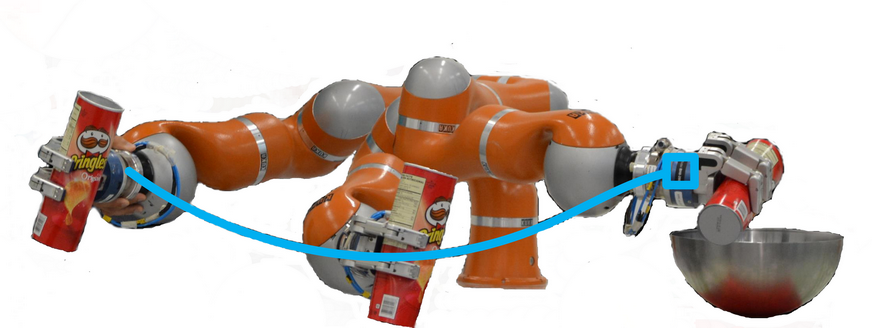
\includegraphics[scale=.155,trim={0 0 0 0cm},clip]{./figures/Without_Obstcle_white_new.png}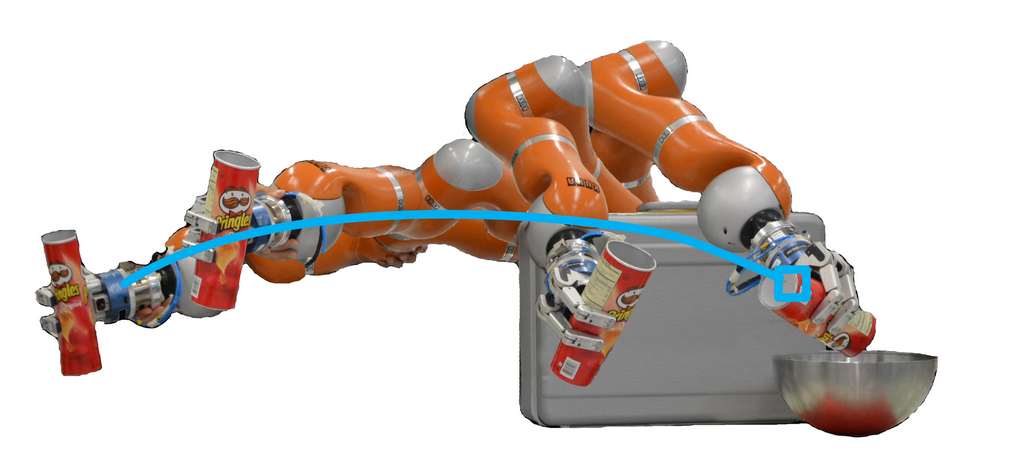
\includegraphics[scale=.125,trim={0 0 0 0cm},clip]{./figures/With_Obstcle.png}
\caption{Two robot motions in \textcolor{orange}{\textbf{joint-space}} accomplishing \textit{similar} behavior in \textcolor{cyan}{\textbf{task-space}} (pouring chips in a bowl). The left example avoids a known obstacle in its workspace, while the right one does not.}
\label{fig:robot_example}
\vspace{-20pt}
\end{figure}


Several approaches have tackled the problem of learning joint-space behaviors with task-space objectives. \cite{calinon2008probabilistic} notably attempted to address this problem by learning separate motion policies in task space and the null space of the Jacobian (which would not affect task-space position), and driving the robot with a weighted sum of the two.  However, this approach does not seek convergence to the desired task-space target and is still reliant on computing the pseudo-inverse Jacobian. \cite{calinon2010learning} and \cite{silverio2017learning} expand on this approach by projecting task-space constraints into joint space using IK, and then learning a joint-space policy that incorporates both task and joint space constraints, but this similarly relies on IK approximations and does not ensure convergence to an attractor.
% FACT-CHECK: is this what Calinon 2009 and Silverio et al. 2017 are doing? They don't ensure convergence, right? TP-GMM never seems to address it ->CORRECT
%\cite{lee2014unifying} learns from demonstration in both joint and task space within the ``thin-plate spline" trajectory warping framework. % but does not propose a dynamical system for generating motions. 
\cite{hersch2008reaching} proposed an approach with similar properties to our desiderata, where two concurrent DS, one in task-space and one in joint-space, are modulated by enforcing kinematic coherence constraints to avoid singularities. The resulting DS avoids singularities through generalization of the pseudo-inverse approximations. However, because the two DS have their own unique attractors, the non-linear interaction between them imposed by the kinematic constraints does not ensure that the combined DS has a unique attractor. This gives rise to spurious attractors or cycles, and thus requires careful tuning to avoid them. 

In this work, we seek to devise an augmented \textbf{J}oint-space \textbf{T}ask-oriented \textbf{D}ynamical \textbf{S}ystem (JT-DS) that not only incorporates task-space attractors, but also avoids the problems generated by pseudo-inverse approximations. To approximate this DS, we further propose an algorithm to learn a set of \emph{behavior synergies}, each of which corresponds to a different stable behavior in joint space, and modulate the use of these synergies throughout joint-space using a learned Linear Parameter Varying (LPV) system. We determine the scheduling parameters for the LPV by finding a \emph{lower-dimensional embedding} of the joint space, which accounts for the variation in the demonstrated motions. We then learn a policy in embedding space for combining our behavior synergies to accurately reconstruct the demonstrated trajectories.
Hence, our dynamical system:
\begin{enumerate}[leftmargin=*]
\item computes a \begin{bf}motion in joint-space\end{bf} that provably and asymptotically converges to a \begin{bf}task-space \end{bf}target.
\item is formulated such that \textbf{joint-space behaviors} can be \textbf{learned} from demonstrations as \textbf{synergies}.
\item can transit through kinematic \textbf{singularities}.
\end{enumerate}


The most similar approach to our proposed DS is the Jacobian transpose (JT) control method \cite{wolovich1984computational} . The JT control is an IK method that yields a dynamical system in joint space
which converges stably over time to a desired end-effector target, without the need for pseudo-inverse computations. It shares some of our approach's advantages: fast computation and provable task-space stability. However, despite some previous work designing velocity adjustments by hand \cite{Shi2016}, this is, to the best of our knowledge the first work to employ a JT system to learn behaviors from demonstrations. Furthermore, by formulating our LPV system on a latent embedding (via dimensionality reduction schemes), we are able to discover meaningful local behavior synergy regions, while being robust to outliers, noise and redundancies that might arise from raw demonstrations. This leads to a compelling improvement in generalization of the demonstrated behavior, as opposed to learning the LPV system solely in joint space. 

This paper is organized as follows. Section \ref{Sec:Prob} formalizes the problem. The proposed dynamical system is introduced in Section \ref{Sec:DS}. In Section \ref{Sec:Learning}, a probabilistic model is introduced to approximate the parameters of the dynamical system. In addition, a convex optimization problem is  formalized to estimate these parameters. In Section \ref{Sec:Exp} we provide a thorough validation of our proposed DS and learning approach. We finalize with a discussion in Section \ref{Sec:Dis}.

%\begin{figure}[t]
%\centering
%
\includegraphics[width=0.95\linewidth,trim={0 20 450 0},clip]{Pic/Schematic.jpg}
%
\includegraphics[width=0.9\linewidth,trim={580 20 0 0},clip]{Pic/Schematic.jpg}
%\caption{ Standard control architecture using Cartesian dynamical systems (DS)\textbf{(top)}  and our proposed approach \textbf{(bottom)}.}
%\label{fig:schematic}
%\end{figure}
\section{Problem Statement} \label{Sec:Prob}
Consider a robotic system with $d$ task-space dimensions and $m$ degrees of freedom. The system is directed via a joint-position or joint-velocity controller. We are further provided with a set of $N$ demonstrated joint-space trajectories $D=\{\{q_{t,n},\dot{q}_{t,n}\}_{t=1,\dots, T_n}\}_{n=1,\dots,N}$, where $T_n$ is the number of the sample points of the $n^{\text{th}}$ demonstration. We refer to the system's joint-space position as $q=\begin{bmatrix} q^1 & \dots & q^m
\end{bmatrix}^T \in \mathbb{R}^m$, and to its task-space target as $x\in \mathbb{R}^d$.\footnote{For pure position targets we consider $d=3$, for position and orientation $d=9$, where the first 3 dimensions correspond to Cartesian position and the remaining 6 correspond to the first and second columns of a rotation matrix $R \in SO(3)$.} The kinematics of the robot are assumed to be known, hence, the robot's forward kinematics are indicated by $x = H(q)$ and its Jacobian is $J(q) = \frac{dx}{dq}\in \mathbb{R}^{d\times m}$.
We wish to formulate a DS $\dot{q} = f(q)$ which satisfies the following two criteria:
\renewcommand{\labelenumi}{(\Roman{enumi})}
\begin{enumerate}
\item The DS must be asymptotically stable\footnote{Unless otherwise specified, ``stability" in this paper always refers to asymptotic stability within the workspace of the robot (in the regions where the Jacobian is full rank), and as such assumes no joint limits. We make no claim to proving global asymptotic stability, which is in fact impossible to achieve in a joint-constrained kinematic system.} with respect to a fixed task-space target $x^*$. This can be expressed by ensuring that the following Lyapunov function\begin{equation}
V(q) = (H(q) - x^*)^T(H(q) - x^*) 
\label{eq:Lyp}
\end{equation}
is stable; i.e. $\dot{V}(q) < 0 ~\forall q\in Q$ and $V(q)=0~ \forall q\in Q^*$ where $Q^*=\{q|H(q)=x^*\wedge q\in Q\}$ and $Q=\{q|q\notin Q^*, J(q) \textit{ is full rank}\}$. $V(\cdot)$ can be thought of as a metric for the task-space distance-to-go.
\item The DS should encapsulate the desired joint-space behaviors such that the following metric is minimized
\begin{equation}
\vspace{-5pt}
e_{total} = \frac{1}{NT_n}\sum_{n=1}^N\sum_{t=0}^{T_n} \left \| \dot{q}_{d; t,n} - f(q_{t,n}) \right \|
\label{eq:optim_error}
\end{equation}
  where $\dot{q}_d$ are the ``true" velocities from the demonstrations, and $f(\cdot)$ is the motion generation policy.
\end{enumerate}

\noindent The error metric \eqref{eq:optim_error} is advantageous in that it mimics the magnitude and direction of the demonstrated motions. This makes the reproduced motion visually most similar to the human definition of ``joint motion style" \cite{gielniak2010stylized}.

\section{Augmented \textbf{J}oint-Space \textbf{T}ask-oriented \textbf{D}ynamical \textbf{S}ystem} \label{Sec:DS}
\label{sec:proposed_system}
To achieve the two criteria presented in \eqref{eq:Lyp} and \eqref{eq:optim_error}, we propose the following DS, which we refer to as the augmented Joint-space Task-oriented DS (JT-DS): 
\begin{equation}
\label{eq:ds}
\dot{q} = f(q) = -\mathcal{A}(q)J^T(q)(H(q) - x^*)
\end{equation}
where  $\mathcal{A}(q)\in \mathbb{R}^{m\times m}$ is constructed using the LPV system paradigm \cite{emedi2016fixed,7439839}. $\mathcal{A}(q) = \sum\limits_{k=1}^{K}\theta_k(\cdot)A_k$ is a linear combination of time-invariant linear matrices $A_k \in \mathbb{R}^{m \times m}$, each of which encodes a ``local joint-space behavior synergy" that shapes the motion in joint-space.  Specifically, the ``local synergy matrices" $A_k$ are joint-space transformations that bias the resulting motion to use particular joints. By modulating each local synergy in time as well as space through the activation functions $\theta_k(\cdot)$ we can generate the desired non-linear joint-space behaviors. Note that in the LPV paradigm $\theta_k(\cdot)$ can be a function of time $t$, ``joint-posture" $q$, an external signal $d(t)$ or a lower-dimensional representation of the joint posture $\phi(q)$. Because we seek a time-invariant controller and know that ``joint-postures" can be accurately represented in a lower-dimensional space, in this work we chose to parametrize $\theta_k(\cdot)$ with $\phi(q)$.

\begin{figure}[!t]
	\centering
	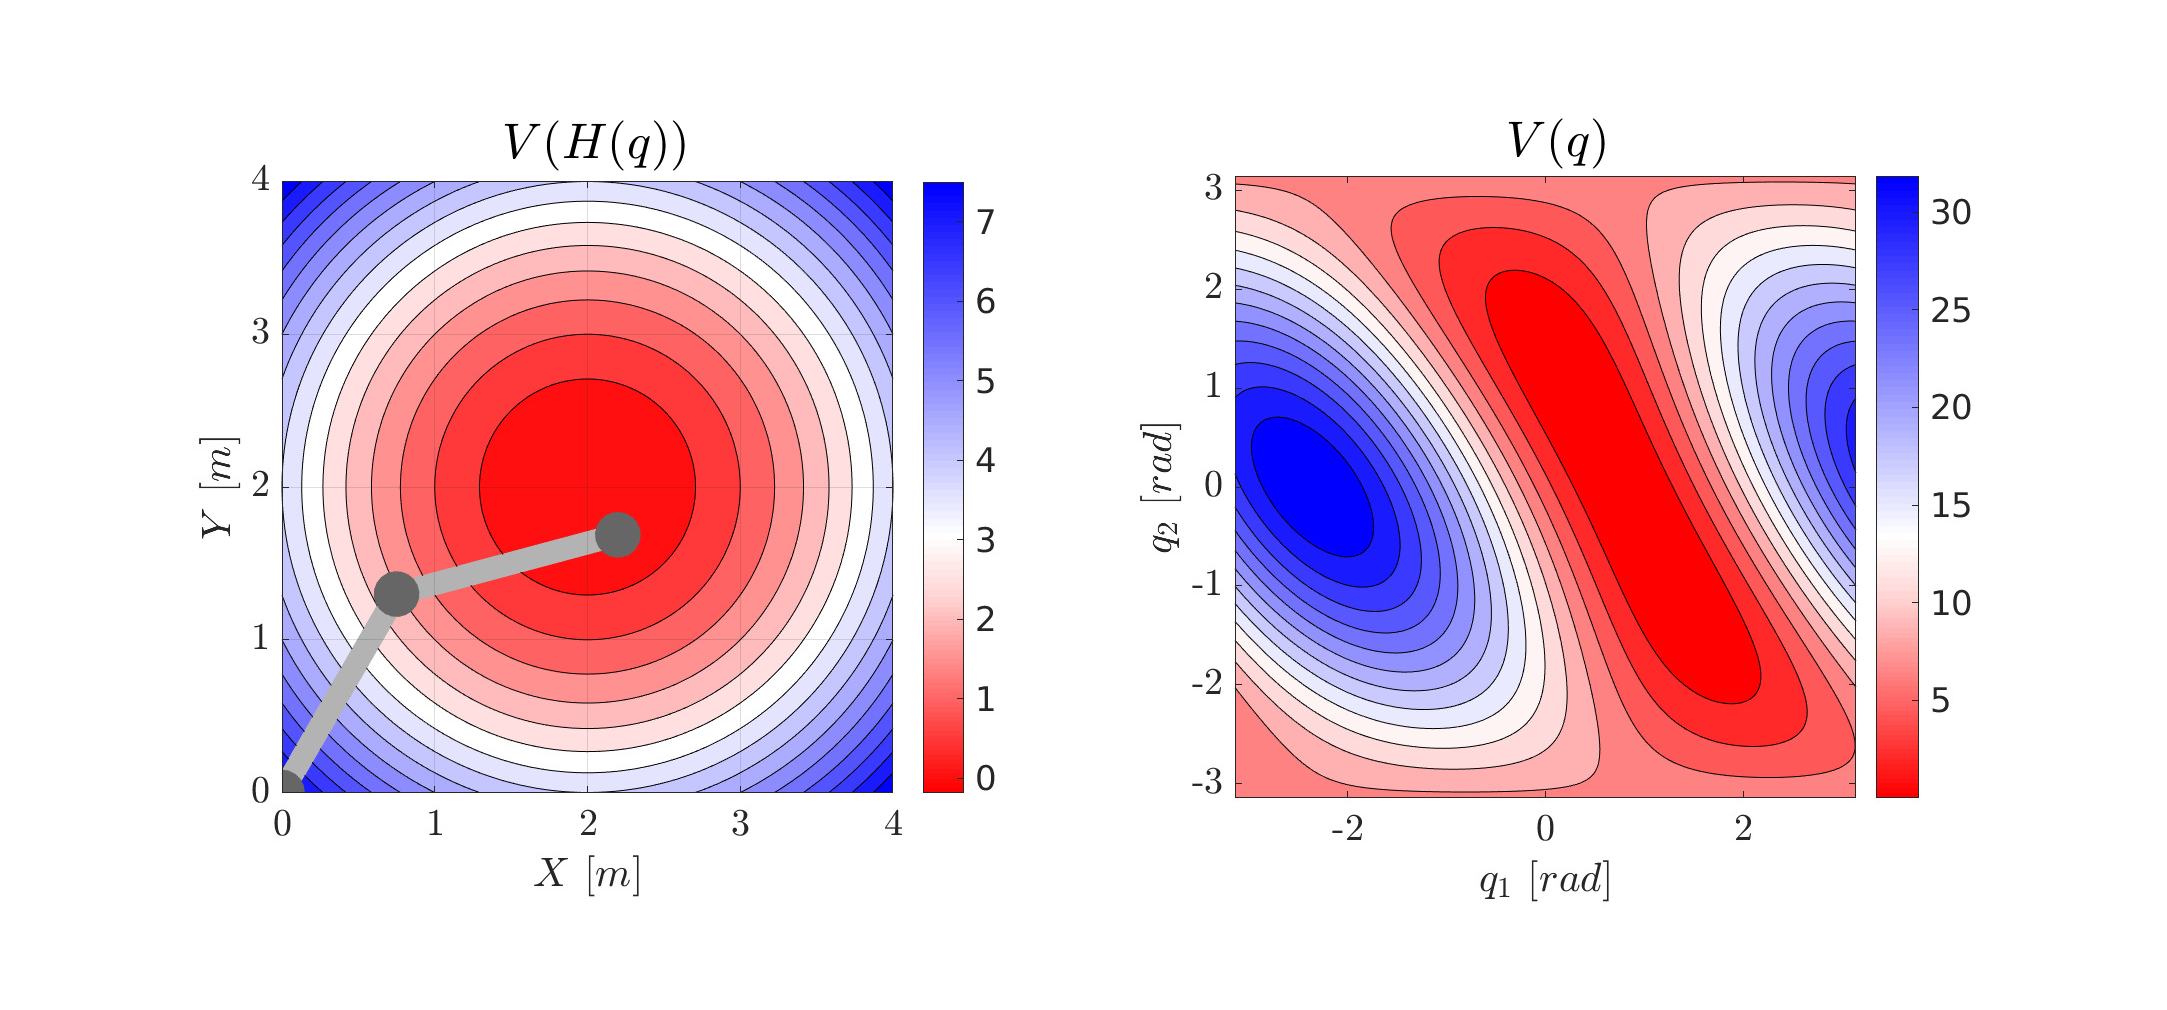
\includegraphics[width=\linewidth,trim={2.5cm 1.75cm 2.5cm 2cm},clip]{./figures/Schematic_final.pdf}
	\caption{Illustration of our task-space and proposed joint-space Lyapunov function. On the left we show the task-space error we are trying to minimize, represented by a potential function for a 2-DOF robot with target $x^*=[2,2]^T$. On the right we show the corresponding Lyapunov function in joint space defined in \eqref{eq:Lyp}. The colors on each plot correspond to each other. One can see how the error, and consequently the \textit{attractive} regions in task-space, have been warped into attractive regions in joint-space.}
	\label{fig:error_schematic}
	\vspace{-15pt}
\end{figure}


Before proving that \eqref{eq:ds} satisfies all of the criteria, one can intuitively understand the control law as follows: $(H(q) - x^*)$ denotes the task-space error wrt. the target\footnote{If the target defines an orientation, this is the Euclidean distance between the two $9$-dimensional position-and-orientation vectors.}. We derive the task-space velocity of a proportional controller minimizing that error by multiplying by $-1$. Then, by multiplying this task-space velocity by the transposed Jacobian $J^T(q)$, it is transformed into a joint-space velocity vector correlated with the error (similar to Jacobian transpose control \cite{wolovich1984computational,sciavicco1988solution}), see Fig. \ref{fig:error_schematic}. The positive definite matrix $\mathcal{A}(q)$ warps the resulting joint-space velocity; Fig. \ref{fig:A_example} illustrates the effects of  $\mathcal{A}(q)$ on the generated motion. Thus the controller can be thought of as a proportional controller in joint space. Lastly, we refer to %the $P$ matrix as the \begin{bf} task augmentation matrix \end{bf}(as it augments the task error, and thus the direction of motion) and 
$\mathcal{A}(q)$ as the \begin{bf} joint augmentation matrix \end{bf} as it augments the outputted joint velocities.
\newtheorem{prop1}{Proposition}
\begin{prop1}
\label{prop:stability}
The DS in \eqref{eq:ds} accomplishes criteria (I) if $ \forall k \in \{1,\dots,K\}  $ the following constraints are met. 
\begin{equation}
\label{eq:first_criteria_stability}
\begin{cases}
\begin{split}
 & A_k \succ 0, & ~~~~ \theta_k(\cdot) \geq 0 \\
\end{split}
\end{cases}
\end{equation}    
\end{prop1}
\vspace{5pt}
\textbf{Proof}: See Appendix \ref{appendix:stability}. $\blacksquare$

Criterion (II) (i.e. encoding specific joint-space behaviors) is achieved by embedding the desired joint-space behavior in the matrices $A_k(q)~ \forall k \in\{1,\dots,K\}$. We describe in the next section an approach to automatically learn the number of matrices $K$, their values and their corresponding activation functions $\theta_k(\cdot)$ from demonstrated data. 

\section{Learning \textbf{J}oint-Space \textbf{T}ask-oriented \textbf{D}ynamical \textbf{S}ystems in Synergy Space} 
\label{Sec:Learning}

The behavior of the JT-DS algorithm can be best understood through the lens of synergy control \cite{7954741}. In robotic synergy control, a robot's movements can be decomposed into a small number of synergies: principal components of the joint-space that are sufficient to accurately recreate the desired robotic behaviors. In our case, the synergies are represented by the matrices $A_1, A_2, \dots, A_k$, and $\mathcal{A}(q)$ represents the resulting motion constructed from a superposition of different synergies (through \eqref{eq:ds}). 

A central question arises: how do we modulate the synergies in different regions to yield our desired behavior? First, we assume that our desired behavior can be efficiently described\footnote{Given some original space $A$ and some behavior policy $\pi_A(a)$ in $A$, we say that an embedding $\phi(\cdot)$ and embedding space $B: \{b = \phi(a) | a \in A\}$ ``efficiently describe" $\pi_A$ if there exists some policy $\pi_B(b)$ in $B$ such that we can deterministically reconstruct $\pi_A(a)$ given $\pi_B(\phi(a))$} using a sub-manifold of the joint-space, called the \emph{embedding space}. We would like to define the robot's policy in embedding space such that in different regions of the space, we will prioritize different synergies. We are thus left with three problems: (I) finding an underlying synergy-space $Z$ in which the behavior can be accurately controlled (defined by a mapping $\phi: Q \rightarrow Z$), (II) finding a policy for modulating the synergies in different regions of the synergy space (defined by $\theta_k(\phi(q))~\forall k\in\{1,\dots,K\}$), and (III) finding parameters for the synergies themselves (defined by $A_k~\forall k\in\{1,\dots,K\}$). Our choice of parameters must also obey the constraints laid out in \eqref{eq:first_criteria_stability}. We thus propose the following 3-step learning procedure:

\begin{figure}[!t]
	\centering
	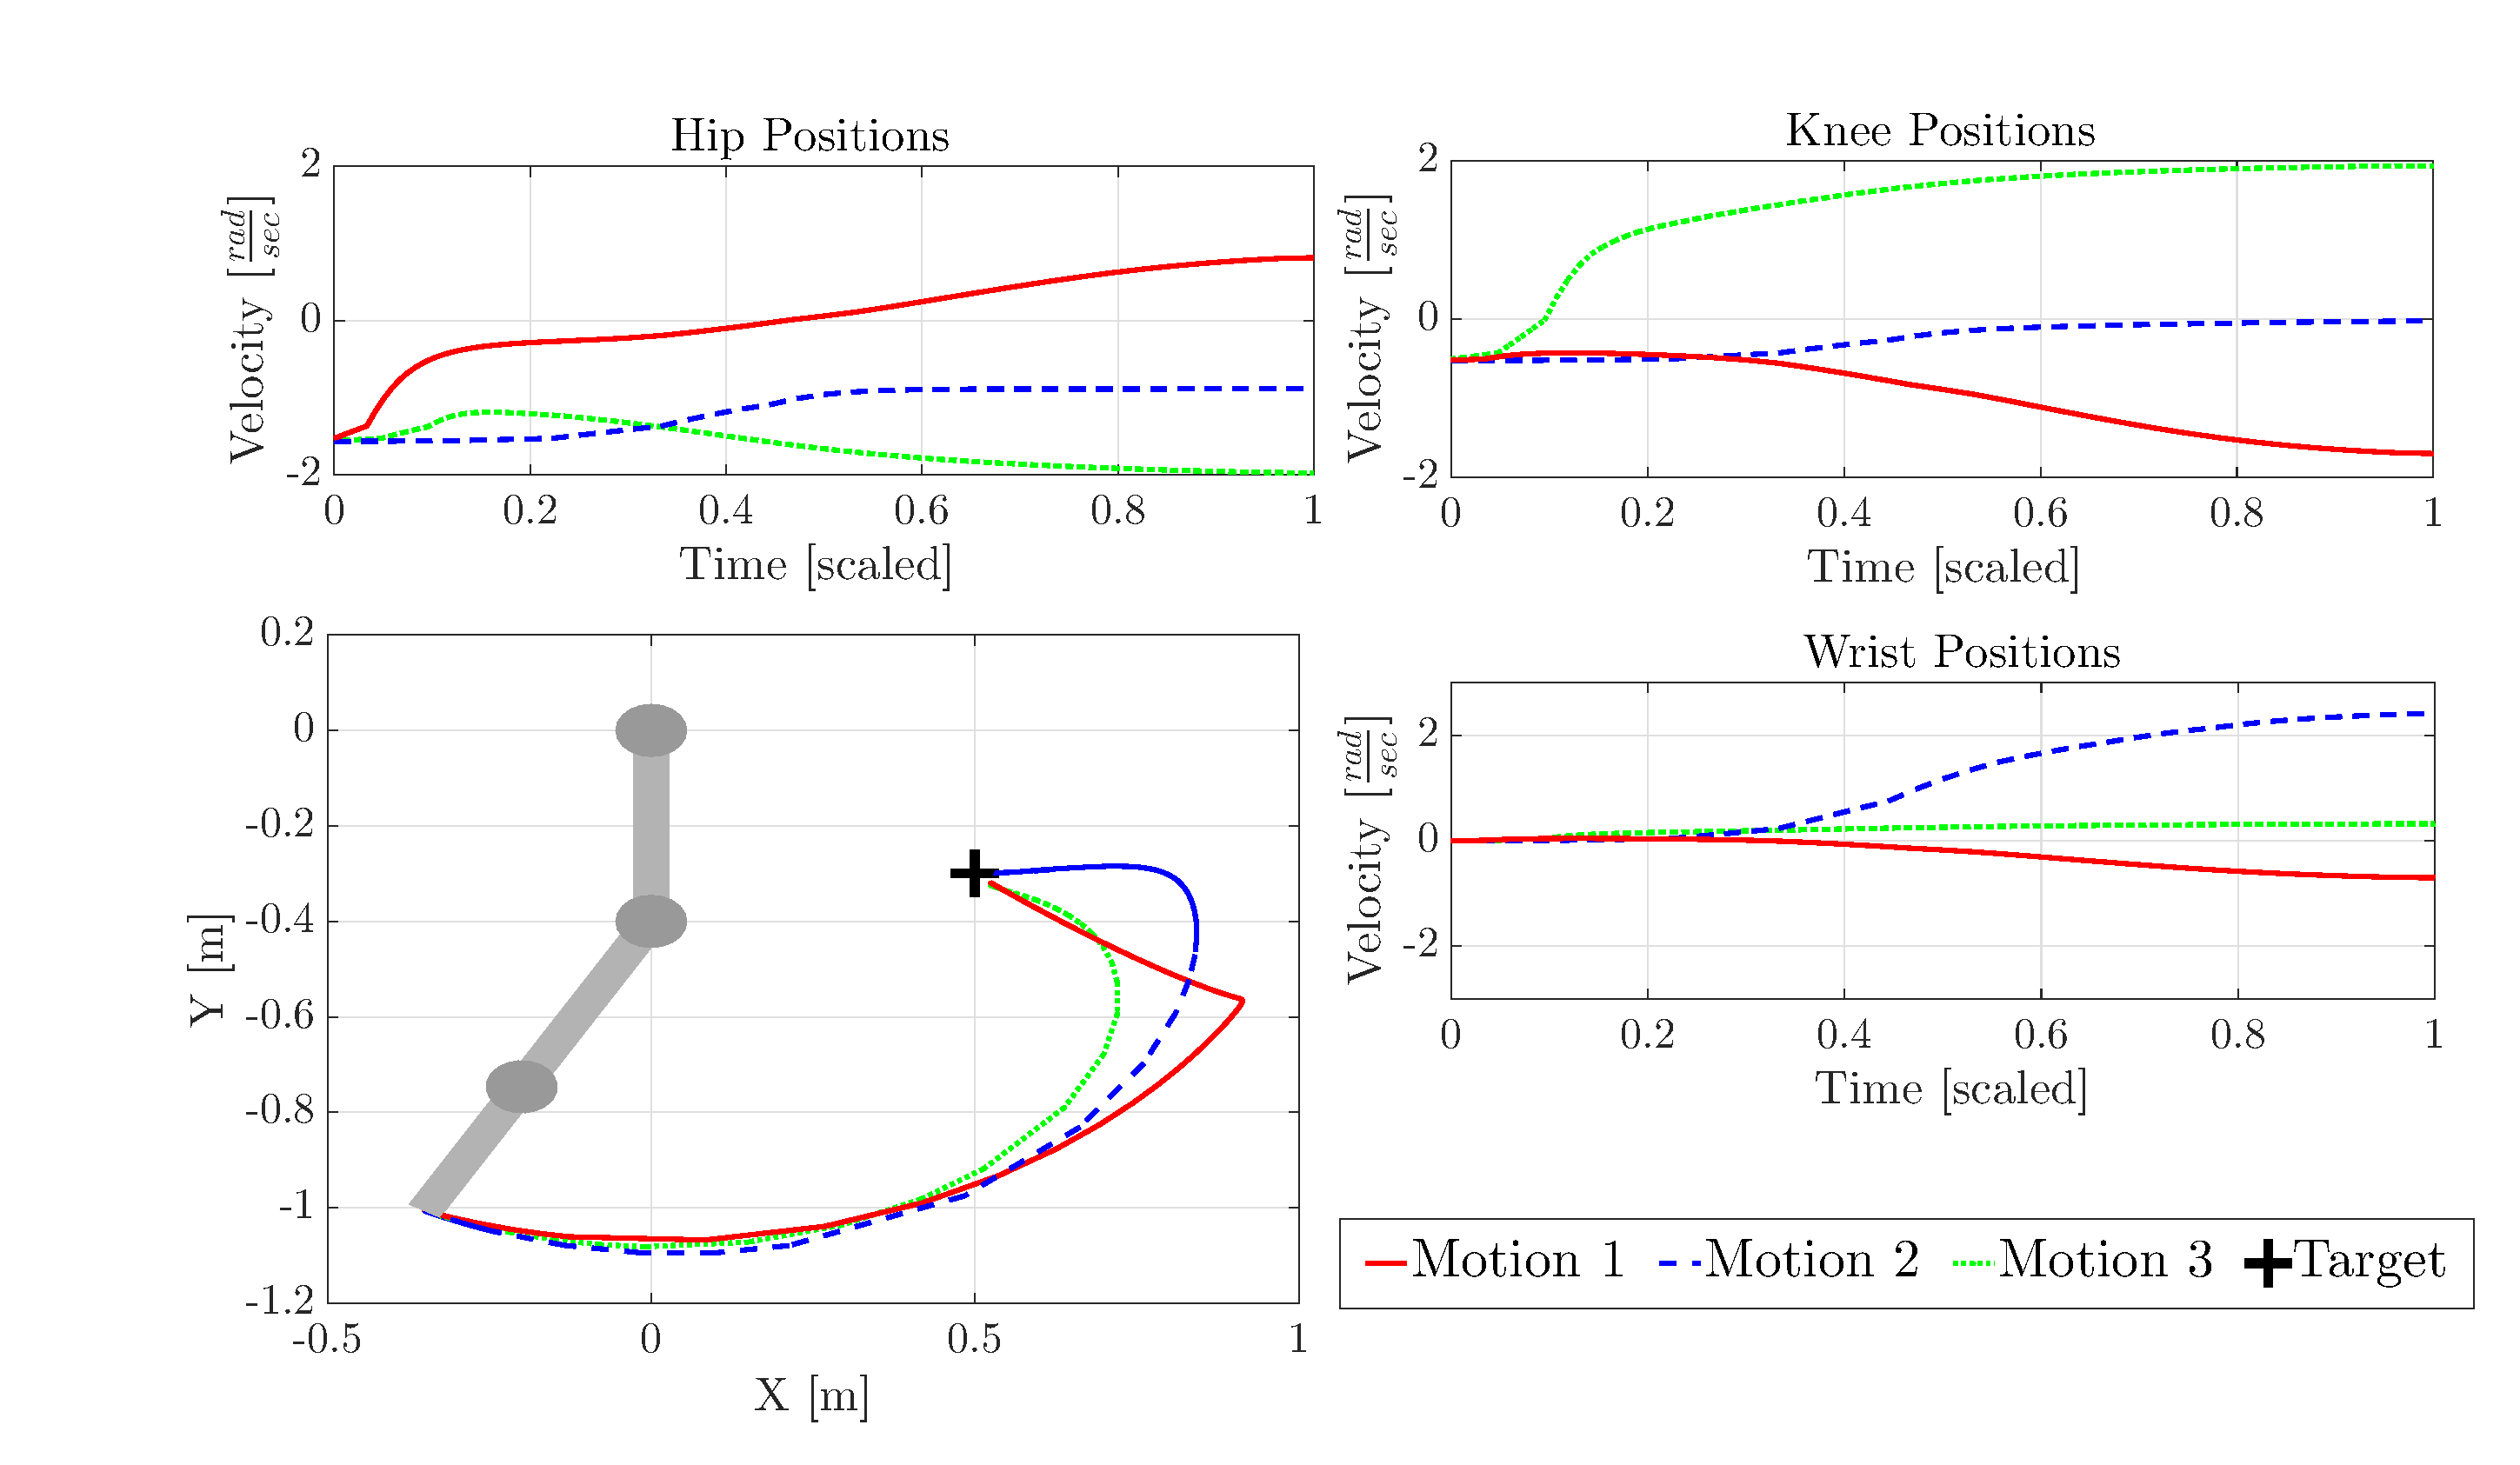
\includegraphics[width=\linewidth]{./figures/A_comparison_positions.pdf}
	\caption{Three example 3-DOF motions (A, B, C), each with a different constant joint augmentation matrix $\mathcal{A}(q)$ (emphasizing the hip, knee, and ankle respectively), A: $\mathcal{A}(q)=diag(5,1,1) $, B: $\mathcal{A}(q)=diag(1,5,1)$, and C: $\mathcal{A}(q)=diag(1,1,5)$. On the left, the task-space traces of each motion. On the right, the time-scaled joint positions of each joint. Each motion tends to use its ``primary" joint most and uses the other available joints to compensate for what the primary joint cannot do.}
	\label{fig:A_example}
	\vspace{-15pt}
\end{figure}


\begin{enumerate}
\item We first construct our embedding, which provides us a lower-dimensional manifold through which to control the robot, by projecting the demonstration data (i.e. collections of joint positions $q \in \mathbb{R}^{m}$) into a lower-dimensional embedding $\phi(q)\in \mathbb{R}^{p\leq m}$. In Section \ref{Sec:Exp} we evaluated Principal Component Analysis (PCA) \cite{jolliffe1986pca} or Kernel PCA (KPCA) with RBF kernel \cite{scholkopf1997kernel}.

\item We then jointly estimate the optimal number $K$ of ``local synergy regions" and the parameters of the scalar functions that determine the activation parameters $\theta_k(\phi(q))$ for weighting these synergies, by fitting a Gaussian Mixture Model (GMM) on the projected joint positions $\phi(q)$ seen in the demonstrations.

\item Once the local synergy regions have been found (described by each of the Gaussian distributions $\theta_k(\phi(q))$), we compute the corresponding joint synergy matrices $A_k~\forall k\in\{1,\dots,K\}$ for each region by formulating a convex optimization problem that finds the optimal set of $A_k$'s that minimize the overall velocity error with respect to the demonstrations \eqref{eq:optim_error}.
\end{enumerate}


\subsection{Embedding Joint Configurations in Low-Dim. Space}
The search for a lower-dimensional embedding of the joint space stems from the desire to identify a simplified coordinate system in which each principal component corresponds to an important source of variation in the demonstrated trajectories, and which is thus suitable for parameterizing the demonstrated behavior. Motor control studies have postulated that human arm motions like reaching or following straight/curved line trajectories, rather than utilizing the full joint space $|q|$, are the result of compromising between planning a straight line in the task space and a straight line in the joint space \cite{Cruse1987humanarm,Okadome1999arm}. This suggests that human arm motion in general tends to move on a plane, and thus can be represented in such a lower-dimensional space. 

In this work, we assume that configurations that are nearby in joint-space should exhibit similar behaviors, and thus it is natural that we choose a low-dimensional embedding that preserves the variance in our demonstrations. To this end, we construct a single global embedding $\phi(q)$ by training dimensionality reduction techniques on the demonstrated trajectories. The learned embedding $\phi(\cdot)$ maps a joint configuration $q \in \mathbb{R}^m$ into a lower-dimensional configuration $z \in \mathbb{R}^p$, where $p < m$. For example, if the shoulder and arm joints are coupled throughout the motion, and $\phi(q)$ were a matrix multiplication (i.e. $\phi(q) = A_p\times q$ for $A_p \in \mathbb{R}^{p\times m}$), it could map the ``shoulder" and ``arm" components of $q$ into a single ``shoulder-arm" component in $\phi(q)$.

\subsection{Discovering Local Behavior Synergies}
The next step is identifying the regions of space in which to activate different synergies. Given the set of projected joint position trajectories $D=\{\{\phi(q_{t,n})\}_{t=1,\dots, T_n}\}_{n=1,\dots,N}$ where $\phi(q_{t,n})$ is the lower-dimensional embedding of $q_{t,n}$, $t$ is the time-step and $N$ is the number of demonstrations, we seek to learn a set of regions of distinct local synergies, each defined by their corresponding activation function $\theta_k(\phi(q))$. Moreover, we would like for $\theta_k(\phi(q))$ to have the following properties: (i) $\theta_k(\phi(\cdot))>0$ and (ii) $\sum_{k=1}^{K}\theta'_k(\phi(q)) = 1$. Such activation functions, also known as scheduling parameters for LPV systems, have been modeled in previous work as probability distributions \cite{7439839, Salehian-RSS-16}. Intuitively, we search for a probabilistic model that ``explains" the variance in the demonstrated trajectories, and treat each cluster as expressing a \textit{local behavior}, which the synergy will then approximate. In this work, we adopt this approach and use a GMM to estimate the joint distribution over the projected joint positions\footnote{It must be noted that, although we present GMM as the approach to estimate the activation parameters, alternative algorithms can be used.}, $p(\phi(q)) = \sum_{k=1}^K\pi_k\mathcal{N}(\phi(q);\mu_k,\Sigma_k)$, where $\pi_k$ are the prior probabilities and $\{\mu_k,\Sigma_k\}$ are the mean and covariance matrices that parametrize the $k$-th multivariate Gaussian distribution. Each distribution represents a local region of projected joint positions $\phi(q)$, and will be used to construct the activation functions $\theta_k$ of the $k$th synergy matrix. We define $\theta_k(\phi(q))$ as $p(k|\phi(q))$:
\begin{equation}
\label{eq:theta}
\theta_k(\phi(q))= \frac{\pi_k\mathcal{N} (\phi(q); \mu_k, \Sigma_k)}{\sum_{k=1}^K \pi_k\mathcal{N} (\phi(q); \mu_k, \Sigma_k)}
\end{equation}
which is the probability of the projected joint-position $\phi(q)$ belonging to the $k$-th local synergy region. Therefore, each synergy region is associated with a Gaussian component of the GMM, cumulatively describing all the synergy regions of the dynamical system. We use the standard Expectation Maximization (EM) training algorithm to estimate the parameters of the GMM \cite{Bilmes98agentle}.  We follow a model selection approach described in Section \ref{Sec:Exp} to find the optimal $K$.

\subsection{Estimating the Synergy Matrices}
Given the parameters of $\theta_k(\phi(q))$ $\forall k \in \{k=1,\dots,K\}$, one can construct $\mathcal{A}(q)$ as a linear combination of local $A_k$ synergy matrices as follows: 
\begin{equation}
\label{eq:A}
\mathcal{A}(q) = \frac{\sum_{k=1}^K A_k \pi_k\mathcal{N}(\phi(q); \mu_k, \Sigma_k)}{\sum_{k=1}^K \pi_k\mathcal{N} (\phi(q); \mu_k, \Sigma_k)}.
\end{equation} 
Notice the resemblance of \eqref{eq:A} to the Nadaraya-Watson kernel estimator \cite{nadaraya1964regress,watson1964regress}\footnote{The Nadaraya-Watson kernel estimator is used to estimate an unknown regressive function $m(x) = \mathbb{E}\{Y|X\}$, which takes the general form of $\widehat{m}(x) = \frac{\sum_{i=1}^n y_i \mathcal{K}(x,x_i)}{\sum_{i=1}^n \mathcal{K}(x,x_i)}$ where $\mathcal{K}(x,x_i)$ is a kernel function denoting the distance or similarity of $x_i$ to the given location $x$. \cite{nadaraya1964regress,watson1964regress}} with a Gaussian pdf as its kernel function. Hence \eqref{eq:A} can be considered a type of kernel estimator, with the key distinction that the weighting functions $\theta_k(\phi(q))$ are not determined by individual points (as in the original Nadaraya-Watson kernel estimator) but by the components of a GMM, similar to the weighting functions derived in Gaussian Mixture Regression (GMR). 

Intuitively, each ``synergy region" is defined by a Gaussian distribution in the lower-dimensional space. The closer the robot is to a region, the more that region's synergy ($A_k$) influences the robot's current joint-space motions. Finding the appropriate synergy matrices $A_k$ to accurately reproduce the observed demonstrations can be reduced to a semidefinite program with the goal of minimizing \eqref{eq:optim_error}. The resulting optimization minimizes the mean squared joint velocity error from \eqref{eq:optim_error}, resulting in a convex semidefinite optimization with a quadratic objective, as follows:
\begin{equation}
\vspace{-10pt}
\begin{aligned}
&\underset{A_1, \dots, A_K}{\text{min}} 
\sum_{n=1}^N\sum_{t=0}^{T_n} \left \| \dot{q}_{d;t,n} - f(q_{t,n}) \right \| \\
& \text{subject to}&\\
&  0 \prec A_k, \; \forall k \in \{1, \dots, K\}. &
\end{aligned}
\label{eq:opt}
\end{equation}
where $f(q_{t,n})$ is calculated by %combining our dynamical system formulation
 \eqref{eq:ds} with \eqref{eq:A}, and $x^*_{n}$ is defined as the endpoint of the $ n^{\text{th}} $ demonstrated trajectory. This optimization is always feasible; the only constraint is that the $A_k$s be independently PSD.



\begin{figure*}[!ht]
  \begin{minipage}[b]{0.31\textwidth}
	\centering	
		\begin{subfigure}[t]{\linewidth}
		\centering
			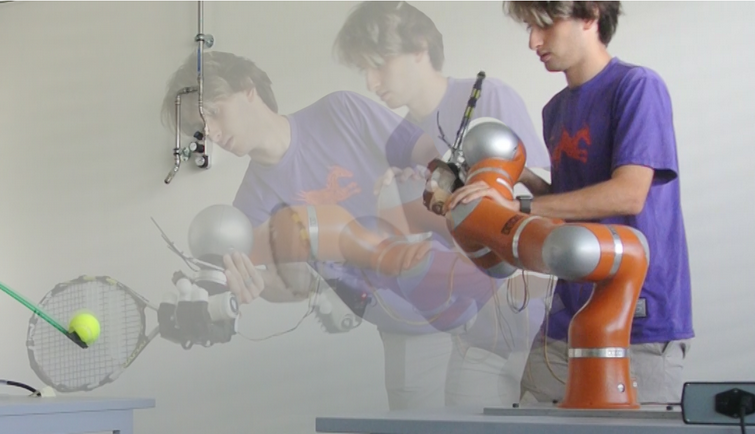
\includegraphics[width=0.5\linewidth]{./figures/forehand_crop.png}\hspace{5pt}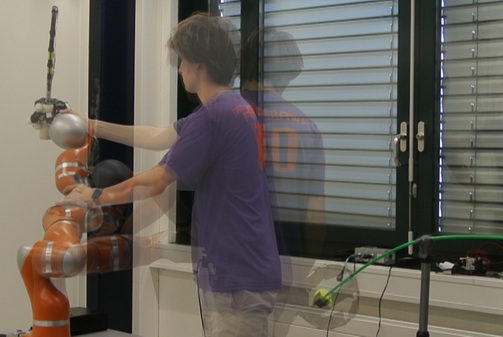
\includegraphics[width=0.43\linewidth]{./figures/backhand_crop.png}
					\caption{Forward/Backward Reaching (1-2).\label{fig:forback}}
		\end{subfigure}
		\begin{subfigure}[t]{\linewidth}
\centering
	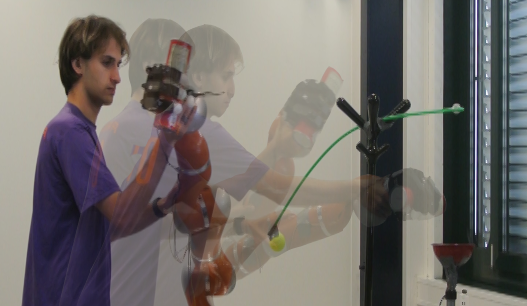
\includegraphics[width=0.45\linewidth]{./figures/pour-free_crop.png}\hspace{5pt}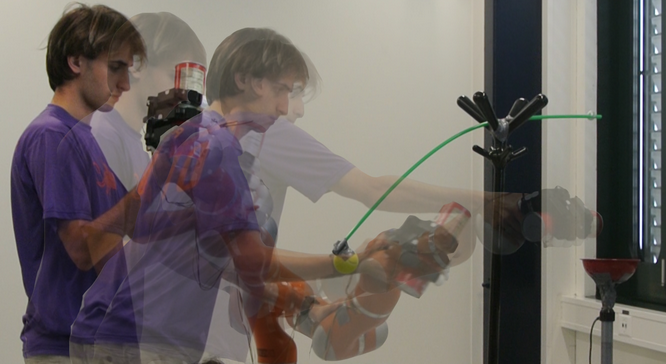
\includegraphics[width=0.477\linewidth]{./figures/pour-obst_crop.png}
						\caption{ Pouring Motions (3-4)}
			\end{subfigure}
			\begin{subfigure}[t]{\linewidth}		
\centering
	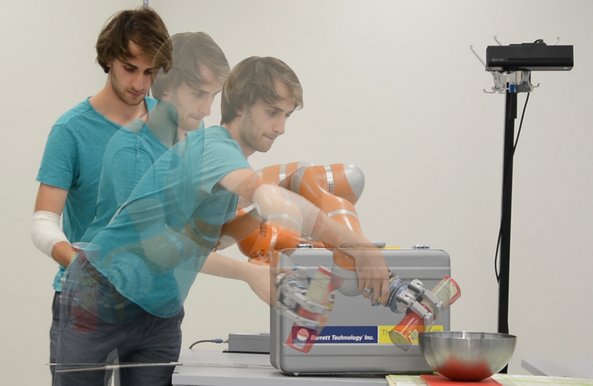
\includegraphics[width=0.45\linewidth]{./figures/pour-obst-2_crop.png}\hspace{5pt}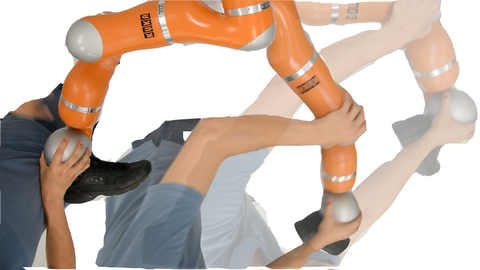
\includegraphics[width=0.5\linewidth]{./figures/footstep.png}
	\caption{ Pouring Motion (5) and Foot-step (6).}
				\end{subfigure}
    \captionof{figure}{Demonstrated Joint-Space Behaviors with Task-Space Targets. \label{fig:behaviors}}
  \end{minipage}
  \hfill
  \begin{minipage}[b]{0.69\textwidth}
    \scriptsize
    \centering
\resizebox{\linewidth}{!}{\begin{tabular}{cc|cc|cc}
    \hline
    \hline
    \multicolumn{1}{c}{\multirow{4}{*}{Behavior Dataset}} & \multicolumn{1}{c}{\multirow{4}{*}{Dim. Red. Approach}} & \multicolumn{4}{c}{\multirow{2}{*}{Optimal Parameters | Joint Velocity RMSE [$rad/s$]}}
	\\  
    & & \multicolumn{1}{c}{\multirow{2}{*}{Optimal $p$}} & \multicolumn{1}{c}{\multirow{2}{*}{Optimal $K$}} & \multicolumn{1}{c}{\multirow{2}{*}{RMSE Train}} & \multicolumn{1}{c}{\multirow{2}{*}{RMSE Test}}	\\ \\ \hline
           
	\multicolumn{1}{c}{\multirow{3}{*}{(1) Forward Reaching}} & None & 7 & 5 $\pm$ (2.90) & \textbf{ 	0.234 $\pm$ (0.027) } & \cellcolor{blue!5} 0.633 $\pm$ (0.458)  \\
    \multicolumn{1}{c}{\multirow{3}{*}{($N=10,M=1424$)}} & PCA & 3.1 $\pm$ (0.316) & 3.8 $\pm$ (1.549) & 0.247 $\pm$ (0.017)  & \cellcolor{blue!10} 0.484 $\pm$ (0.263) \\	
		& K-PCA ($\sigma_{opt} = 5.111$) & \textbf{3 $\pm$ (0)} & \textbf{3.5 $\pm$ (1.204)} & 0.2532 $\pm$ (0.019) & \cellcolor{blue!15} 0.385 $\pm$ (0.098)  \\
		\hline
	\multicolumn{1}{c}{\multirow{3}{*}{(2) Backward Reaching}} & None & 7 & 5.8 $\pm$ (2.097) &\textbf{ 0.281 $\pm$ (0.015)} &  \cellcolor{blue!5} 0.647 $\pm$ (0.354)  \\
		    \multicolumn{1}{c}{\multirow{3}{*}{($N=11,M=1223$)}} & PCA & 4.4 $\pm$ (0.516) & 6 $\pm$ (3.091) & 0.282 $\pm$ (0.044) & \cellcolor{blue!10} 0.466 $\pm$ (0.102) \\	
			& K-PCA ($\sigma_{opt} = 6.238$) & \textbf{3.5 $\pm$ (0.5)} & \textbf{3.1 $\pm$ (0.3)} & 0.319 $\pm$ (0.025) & \cellcolor{blue!15} 0.482 $\pm$ (0.114)   \\
			\hline
	\multicolumn{1}{c}{\multirow{3}{*}{(3) Pouring - Free}} & None & 7 &  4.6 $\pm$ (1.897) & \textbf{0.181 $\pm$ (0.019)} & 1.099 $\pm$ (1.140) \\
   \multicolumn{1}{c}{\multirow{3}{*}{($N=9,M=1032$)}} & PCA & 2.6 $\pm$ (0.5164) & 4 $\pm$ (1.054) &  0.186 $\pm$ (0.026)  & \cellcolor{blue!10} 0.419 $\pm$ (0.119) \\	
	& K-PCA ($\sigma_{opt} = 3.92$) & \textbf{2} & \textbf{3.5 $\pm$ (0.5)} & 0.183 $\pm$ (0.0204) & \cellcolor{blue!15} 0.397 $\pm$ (0.105)   \\
				\hline
	\multicolumn{1}{c}{\multirow{3}{*}{(4) Pouring - Obstacle 1}} & None & 7 & 7 $\pm$ (2.357) & \textbf{0.296 $\pm$ (0.029)} & 0.984 $\pm$ (0.55) \\
   \multicolumn{1}{c}{\multirow{3}{*}{($N=11,M=1232$)}} & PCA & 3.9 $\pm$ (0.316) & 3.6 $\pm$ (0.699) & 0.321 $\pm$ (0.028) & \cellcolor{blue!10} 0.402 $\pm$ (0.0587) \\	
				& K-PCA ($\sigma_{opt} = 7.695$) & \textbf{ 3 } & \textbf{ 3.2 $\pm$ (0.4) } & 0.311 $\pm$ (0.011) & \cellcolor{blue!15} 0.388 $\pm$ (0.040)   \\
				\hline	
	\multicolumn{1}{c}{\multirow{3}{*}{(5) Pouring - Obstacle 2}} & None & 7 & 4.1 $\pm$ (1.7288) & \textbf{ 0.1242 $\pm$ (0.0169) } & 1.0907 $\pm$ (1.0686) \\
   \multicolumn{1}{c}{\multirow{3}{*}{($N=7,M=1406$)}} & PCA & \textbf{ 2.8 $\pm$ 0.4216 } & 3.6 $\pm$ (1.8974) & 0.1345 $\pm$ (0.0218) & \cellcolor{blue!10} 0.693 $\pm$ (1.0541) \\	
	& K-PCA ($\sigma_{opt} = 2.86$) & 3.4 $\pm$ (0.4899) & \textbf{3.1 $\pm$ (0.3)} & 0.1345 $\pm$ (0.0182) & \cellcolor{blue!15} 0.4028 $\pm$ (0.1377)  \\
				\hline
	\multicolumn{1}{c}{\multirow{3}{*}{(6) Foot Step}} & None & 7 & 4.2 $\pm$ (1.4757) & \textbf{ 0.1396 $\pm$ (0.0252) } & 1.0697 $\pm$ (0.6574)  \\
	\multicolumn{1}{c}{\multirow{3}{*}{($N=8,M=1058$)}} & PCA & \textbf{1} & 3.1 $\pm$ (0.3162) & 0.1494 $\pm$ (0.0143) & \cellcolor{blue!10}  0.2578 $\pm$ (0.0795) \\	
	& K-PCA ($\sigma_{opt} = 1.513$) & 2 & \textbf{3} &  0.1557 $\pm$ (0.0116) & \cellcolor{blue!15} 0.2271 $\pm$ (0.0466)   \\
				\hline		
	\multicolumn{1}{c}{\multirow{3}{*}{(7) Singularity Motions}} & None & 7 & 6.4 $\pm$ (1.5055) & \textbf{0.048 $\pm$ (0.0158)} & 0.2365 $\pm$ (0.0768)  \\
    \multicolumn{1}{c}{\multirow{3}{*}{($N=10,M=1467$)}} & PCA & \textbf{1.9 $\pm$ (0.3162)} & 5.7 $\pm$ (1.6364) &  0.0503 $\pm$ (0.0153) & \cellcolor{blue!10} 0.1802 $\pm$ (0.0748) \\	
	& K-PCA ($\sigma_{opt} = 1.769$) & 3.9 $\pm$ (0.3) & \textbf{5.2 $\pm$ (2.1817)} & 0.0593 $\pm$ (0.0122) & \cellcolor{blue!15} 0.1276 $\pm$ (0.0591)   \\ \hline\hline
\end{tabular}}
      \captionof{table}{\scriptsize Performance Comparison of Learning Approach with different Dim. Red. Schemes. We present the \texttt{mean(std)} for the optimal $p$, $K$ and joint-velocity RMSE on training and testing set, found for every learning scheme over 10 runs. $M = \sum_{n=1}^{N}T_n$.\label{tab:learning}}.
    \end{minipage}
    \vspace{-20pt}
\end{figure*}

\section{Experimental Validation} 
\label{Sec:Exp}
\subsection{JT-DS Learning Performance  Evaluation}
To evaluate the proposed JT-DS learning algorithm we collected kinesthetic demonstrations on a 7-DOF KUKA LWR 4+ robot arm, for 7 different tasks (see Table \ref{tab:learning} and Fig. \ref{fig:behaviors}) which require mimicking the demonstrated joint-space behavior while reaching for a single target in task space:
\begin{itemize}[leftmargin=*]
\item \textit{(1-2) Forward/Backward reaching:} We guide the robot in forward and backward reaching motions towards a specific target in task-space with joint-space trajectories mimicking forehand/backhand strokes as shown in Fig. \ref{fig:forback}.  
\item \textit{(3-5) Pouring motions:} We guide the robot to emulate pouring motions with three different environmental constraints, leading to different joint-space trajectories. The first is without an obstacle in the workspace. The second is with an obstacle in the upper hemisphere of the workspace, where the human is seen folding the elbow and lowering the shoulder of the robot arm to avoid the obstacle. The third instance is with an obstacle in the lower hemisphere, and now the human raises the shoulder to avoid it.
\item \textit{(6) Footstep-like motion:} We demonstrate a footstep motion which begins with a straight leg, moving through a singularity, and finally bringing the knee up.
\item \textit{(7) Singularity motions:} Movement was constrained to the boundary of the workspace by fixing $ q^i=0~\forall i\in\{3,\dots,7\}$, the second joint was fixed to $q^2\in\{10^\circ,20^\circ,\dots,100^\circ\}$, and only the first joint was moved by a human. This restricted the motion to a series of arcs of different radii along the robot's motion boundary.  
\end{itemize}

\noindent   The recordings are collected at a rate of 500 Hz. However, our learning approach does not require such a dense representation of the trajectories, hence we down-sample them to 25 Hz. By performing our evaluation on all these datasets, we seek to: 

\begin{enumerate}[leftmargin=*]
\item Verify that the learned \textit{behavior synergies} are mimicking the demonstrated joint-space behaviors and generalize them to new initial joint configurations.
\item Analyze the role of dimensionality reduction in our proposed approach and further find the method which yields the best trade-off between accuracy and model complexity; i.e. the least number of dimensions $p$ to represent our activation function $\theta(\phi(q))$ and the least number of local behavior synergies $K$.
\end{enumerate}
We thus evaluate three learning approaches with different dimensionality reduction algorithms: (1) None, (2) PCA and (3) K-PCA with RBF kernel.
We perform 10-fold cross-validation on all datasets, for each learning approach, with a training/testing ratio of $60 \%$. To evaluate performance, we take the square root of the MSE defined in \eqref{eq:optim_error}, which we refer to as the joint-velocity RMSE. 


\begin{figure*}[t]
	\vspace{-0.05cm}
	\begin{subfigure}[t]{0.42\linewidth}
		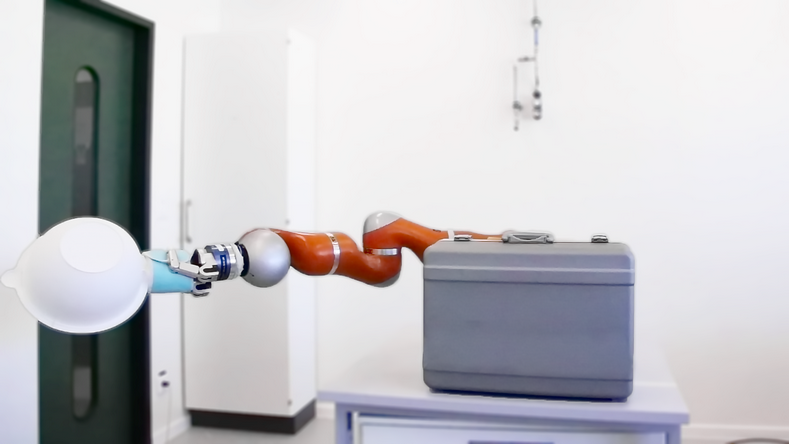
\includegraphics[width=0.45\linewidth]{./figures/Luggage1.png}
		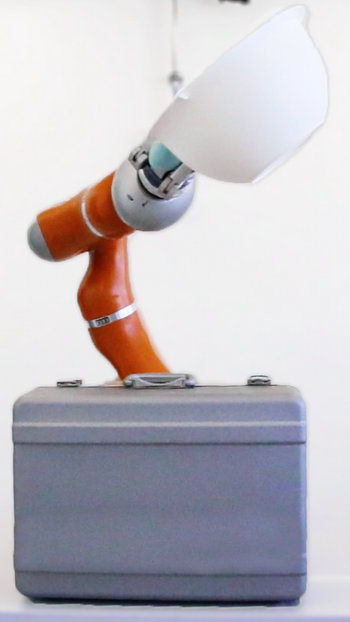
\includegraphics[width=0.143\linewidth]{./figures/Luggage2.png}
		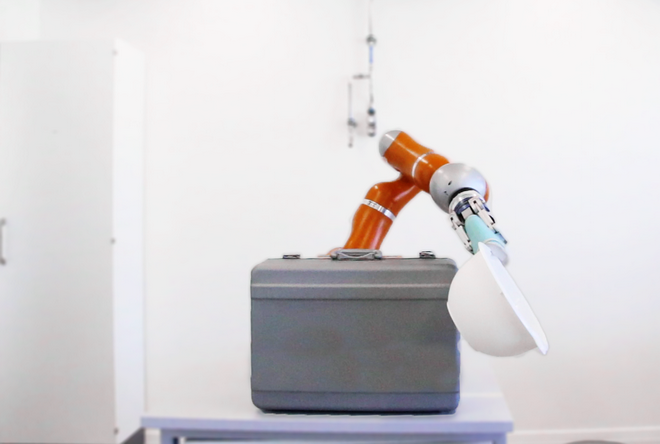
\includegraphics[width=0.377\linewidth]{./figures/Luggage3.png}
		\caption{Execution of Pour Obstacle 2 learned through JT-DS.}
		\label{fig:snapshot:a}
	\end{subfigure}
	\begin{subfigure}[t]{0.567\linewidth}
		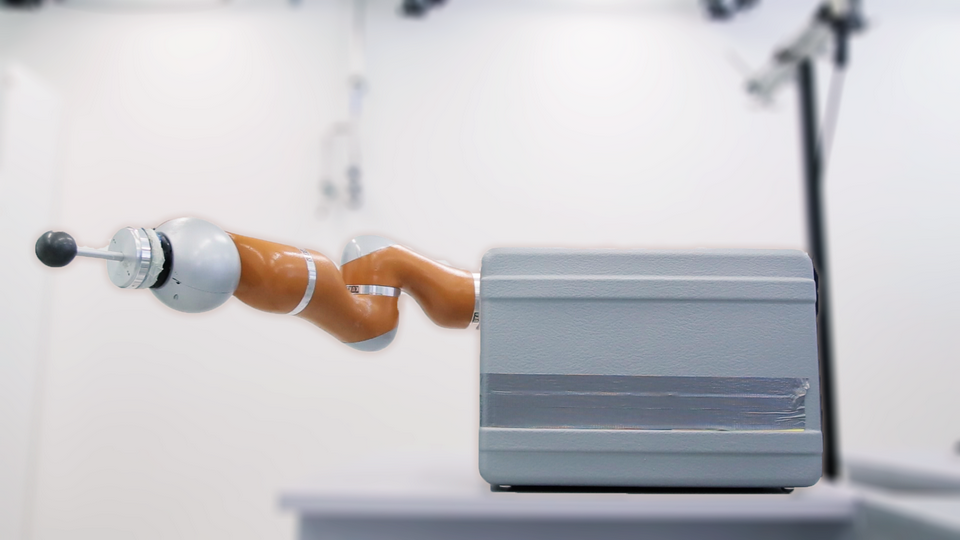
\includegraphics[width=0.33\linewidth]{./figures/Luggage4_SEDS.png}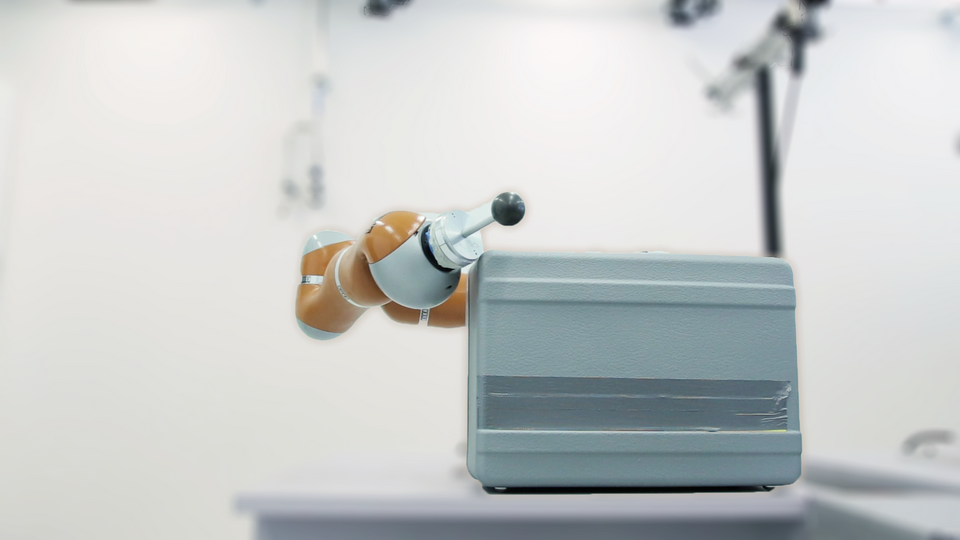
\includegraphics[width=0.33\linewidth]{./figures/Luggage2_SEDS.png}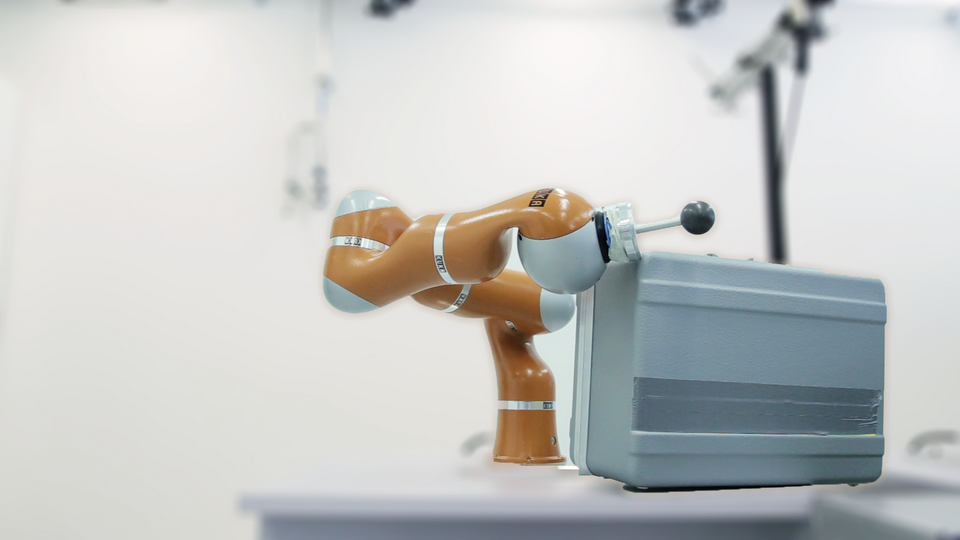
\includegraphics[width=0.33\linewidth]{./figures/Luggage3_SEDS.png}
		\caption{Execution of Pour Obstacle 2 learned through SEDS.}
		\label{fig:snapshot:b}
	\end{subfigure}\\	
	\caption{Snapshots of the robot experiments. A corresponding video is available on-line \href{https://youtu.be/mv9u5DgIEtw}{[https://youtu.be/mv9u5DgIEtw]}.}
	\label{fig:snapshot}
	\vspace{-10pt}
\end{figure*}


Performing such cross-validation in our case is not trivial, as our $\mathcal{A}(q)$ formulation has several hyper-parameters: the dimensionality $p$ of our lower-dimensional embedding $\phi(q)$ and the number of local behavior synergies $K$. Moreover, when using K-PCA (with RBF kernel $k(q,q') = \exp(-\frac{||q-q'||^2}{2\sigma^2})$) we must also find the optimal width $\sigma$. Thus, for each fold and each learning approach we find the optimal hyper-parameters $p$, $K$ and $\sigma$ (when applicable), as follows:
\begin{enumerate}[leftmargin=*]
\item \textit{$p$ for PCA:} We choose $p$ such that the projection is capable of explaining $95\%$ of the variance in the data.
\item \textit{$p$ and $\sigma$ for K-PCA:} The interaction of these two parameters plays a major roll in the resulting projection obtained from K-PCA. Hence, we do a grid search on a log-spaced range of $\sigma_{range} = [\sigma_{min}:\sigma_{max}]$ values, where 
$\sigma_{min} = \frac{1}{\kappa\sqrt{2}} \underset{i \in M,j\in M}{\max}\{||q_i - q_j||^2\}$ and $\sigma_{max} = \frac{2\kappa}{\sqrt{2}} \underset{i \in M,j\in M}{\max}\{||q_i - q_j||^2\}$ for $\kappa = cte.$ This yields a feasible range for $\sigma$ that is guided by the pairwise Euclidean distances between all points in the dataset. Moreover, K-PCA is not limited to providing a $p \ll m$, in fact it can generate $p \le M$. This is a nuisance as in our datasets $M\approx1000$. To alleviate this we truncate $\sigma_{range}$ by computing the explained variance of the eigenvectors in feature space for different values of  $\sigma \in \sigma_{range}$. We then remove $\sigma$ values from $\sigma_{range}$ whose number of \textit{optimal} eigenvectors $p > m$ and resample it. By doing this procedure, we can ensure that for all values in truncated $\bar{\sigma}_{range}$ we will obtain $p \le m$. We then choose $\sigma_{opt}$ by running 10-fold cross-validation for all $\sigma \in \bar{\sigma}_{range}$. 
\item \textit{$K$ for GMM:} We choose the optimal number of components $K$, by evaluating and selecting the best resulting model using the Bayesian Information Criterion (BIC) \cite{Bishop:PRM:2006}. Typically, one chooses the optimal $K$ manually, by visually identifying the point at which the BIC curve produced from $K_{range}$ stops changing or plateaus. To automate this process, we devised an approach which selects the optimal $K$ as the one which yields the highest inflection point on the second order derivative of the BIC curve.
\end{enumerate}


Once these optimal hyper-parameters are estimated for each fold, we solve for the convex optimization problem in order to find our synergy matrices $A$'s which best minimize the objective function \eqref{eq:opt}. We then select the initial joint configuration $q_0$ and target in task-space $x^*$ from each training/testing dataset, simulate the joint-space trajectories $\{\dot{q_1},\dots,\dot{q_T}\}$, with our learned $\mathcal{A}(q)$, and compute the joint-velocity RMSE between these simulations and the training/testing trajectories, as reported in Table \ref{tab:learning}.

As can be seen, for all datasets there is a significant increase in performance on the testing sets when using either dimensionality reduction (DR) approaches. This suggests that using DR to encode our activation functions $\theta_k$ in a lower-dimensional space $\phi(q)$ yields better generalization capabilities than encoding the behaviors in using the original $q$. This is most notable for the three pouring motions, where the joint-velocity RMSE testing error for a JT-DS model learned without DR is an order of magnitude higher than with DR. Such an error indicates that the demonstrated joint-behavior was over-fitted on the training set, which is also exhibited in the higher number of $K$ needed to represent the motion without DR. For all datasets, the DR methods provided $p < m/2$, either comparable or less number of local behaviors synergies $K$ and better RMSE errors on testing sets as opposed to no DR. By finding a lower-dimensional manifold to represent the joint trajectories, we are getting rid of outliers, noise and redundancies that might arise from the raw joint demonstrations. Hence, through DR we are capable of robustly extracting the local behavior synergies from raw demonstrations. 
\begin{figure}[t]
	\begin{minipage}[b]{\linewidth}
		\centering
		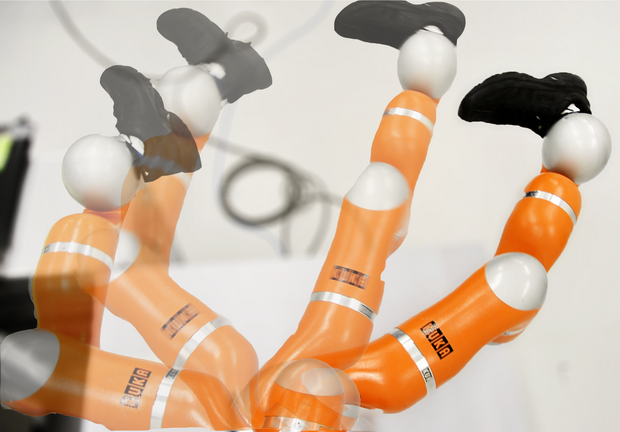
\includegraphics[angle=180,origin=c,width=0.5\linewidth]{./figures/footstep_execution_crop.png}\hspace{5pt}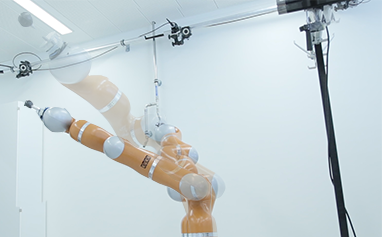
\includegraphics[width=0.4\linewidth]{../new-pics/singularity_crop.png}
		\caption{Execution of \textit{problematic} joint-space behaviors learned through JT-DS: (left) Foot step-like motion and (right) Singularity motions.}
		\label{fig:snapshot:c}
	\end{minipage}
	\begin{minipage}[b]{\linewidth}
		\centering
		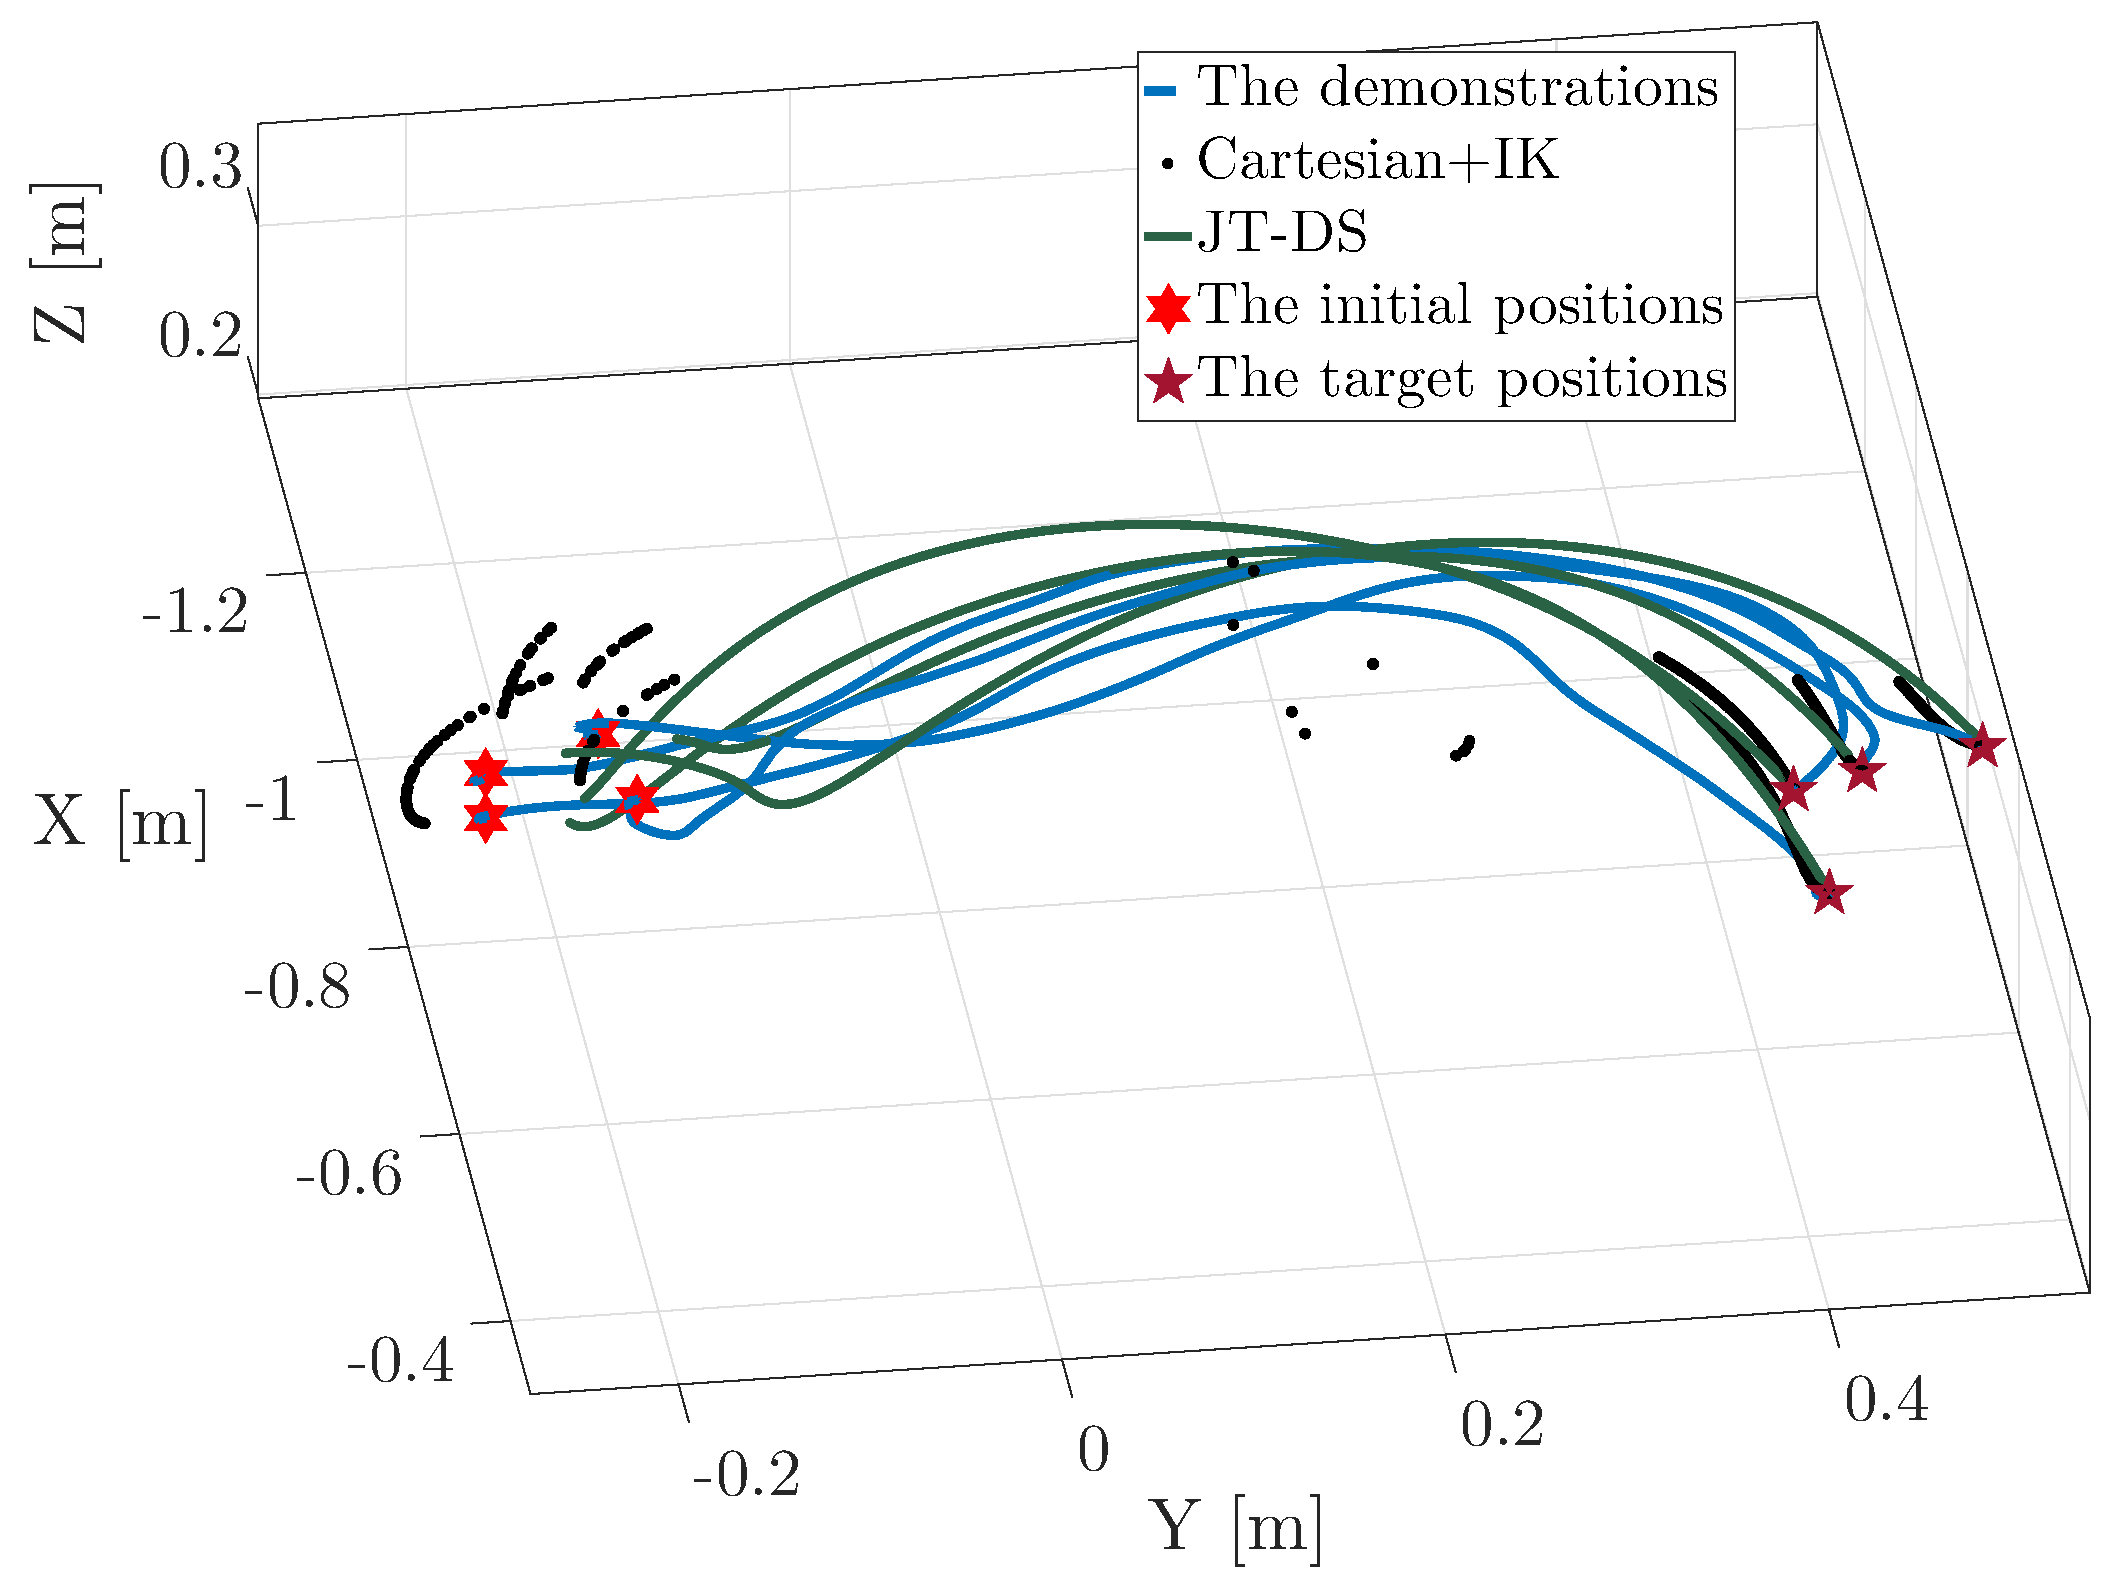
\includegraphics[width=0.7\linewidth]{./figures/Foot.pdf}
		\caption{End-effector trajectories for the footstep motion in Cartesian space. The JT-DS motion moves smoothly closely resembles the demonstrated trajectories. On the other hand, the SEDS-based Cartesian motion generator (whose values here are simulated because they can not physically executable) quickly becomes unstable, as evidenced by the dotted paths starting on the left side and abruptly disappearing. \label{fig:foot}}
		\vspace{-10pt}
	\end{minipage}
	\vspace{-20pt}
\end{figure}


Both PCA and K-PCA yield comparable results, with K-PCA providing a slight improvement on some datasets. This suggests that perhaps a linear DR method might be sufficient for such tasks. However, if we seek to maximize accuracy a non-linear DR method should be employed. One of the drawbacks of K-PCA is its computational complexity for out-of-sample evaluations, which involves computing the kernel function between the new data-point and all the samples $M$. This is, however, not so taxing for our method as our datasets range in $M\approx1000$ and in previous work \cite{Mirrazavi:IJRR:2017} we have experimentally found that evaluating $<3000$ RBF kernel computations (on a 3.4-GHz i7 PC with 8GB RAM)) in a control-loop with 2ms rate is feasible. If one requires extremely fast computation; i.e. a control-loop rate of $<2$ms then PCA should be used as opposed to K-PCA.


\textit{Implementation Details:} The learning pipeline is implemented in MATLAB. We used the Matlab Toolbox for Dimensionality Reduction \cite{Maaten08dimensionalityreduction} for implementations of PCA, K-PCA and its out-of-sample extension. The YALMIP framework \cite{lofberg2004yalmip} was used to solve the definite convex optimization problem. Source code for the entire learning pipeline and simulated behavior on multi-DOF robot arms can be found in:
\footnotesize  \centerline{\underline{\url{https://github.com/epfl-lasa/JT-DS-Learning}}}
\normalsize
For execution of the learnt JT-DS models on a real 7-DOF the KUKA LWR 4+ robot arm, we provide the following code in C++:
\footnotesize \underline{\url{https://github.com/epfl-lasa/JT-DS-lib}}\\
\normalsize
The robot is controlled on the joint position level (linearly interpolating from joint velocities computed from JT-DS) at a rate of $ 500 $ Hz. The resultant joint angles are filtered by a critically damped filter to avoid high torques.
\subsection{JT-DS Execution Performance Evaluation}
We now seek to elucidate the distinctive properties of our JT-DS model by comparing its performance to a DS-based Cartesian motion generator + IK solver approach for behaviors \textit{(5-7)}. For the Cartesian motion generator we use the SEDS (Stable Estimator of Dynamical Systems) approach \cite{khansari2011learning} which learns an asymptotically stable DS in Cartesian space from demonstrations. We then generate joint trajectories through a damped least square IK solver. From hereon we refer to this approach as SEDS+IK.

\subsubsection{Following Desired Joint and Task-Based Behaviors}
We compare tracking capabilities of our JT-DS method with those of SEDS+IK for behaviors \textit{(5)} and \textit{(6)}. In Fig. \ref{fig:snapshot:a} and \ref{fig:snapshot:b} we can qualitatively see the difference between these two approaches for behavior \textit{(5)}. The JT-DS algorithm mimicked the joint-space behavior of the demonstration (e.g. folding the elbow, raising the shoulder), successfully avoiding the obstacle while still converging to the desired Cartesian position. Meanwhile, SEDS+IK only learned the demonstrated behavior in task-space; it is incapable of constraining motion in joint-space. This ultimately led to one of its joints colliding with the obstacle. It should be noted that the JT-DS motion did not follow the demonstrations in task-space very closely (as expected), but did ultimately converge to its target position. For the foot-step behavior \textit{(6)} JT-DS followed the demonstrations closely, while SEDS became unstable in the singularity (Fig. \ref{fig:snapshot:c} and \ref{fig:foot}). This demonstrates the JT-DS algorithm's ability to move cleanly in and out of singularities.

\subsubsection{Transiting through singular configurations}
One of the main advantages of the proposed DS is its ability to generate accurate paths in classical singular configurations. To evaluate this we generated behavior \textit{(7)}; i.e. joint-trajectories that transit entirely within a classic kinematic singularity. Fig. \ref{fig:Sin} shows the \textit{demonstrated} motions and the motion  \textit{generated} by JT-DS \eqref{eq:ds}. The algorithm never requires the pseudo-inverse of the Jacobian matrix, so the generated motion perfectly follows the demonstrations throughout the workspace boundary. In Fig. \ref{fig:snapshot:c} we show the learnt singular motion successfully  executed on the real robot.

\section{Discussion} 
\label{Sec:Dis}
In this paper, we have presented a dynamical system in joint space that is provably asymptotically stable in task space to a fixed target while replicating demonstrated joint-space behaviors. The desired motions are fast to compute, and smoothly handle singularities by avoiding the pseudo-inverse Jacobian.  We showed the system's ability to learn different joint-space behaviors on a robotic platform.

One of the most important points when validating a learning from demonstration method is to evaluate the system's behavior away from demonstrations.
 When the current joint configuration is far from any of the local synergy regions, computing the activation parameters $\theta_k(\cdot)$ becomes numerically infeasible (all the Gaussians in \eqref{eq:A} $\rightarrow 0$), and so we default to $\mathcal{A} = \frac{1}{K}\sum\limits_{k=1}^{K}A_k$, which still guarantees that the robot moves towards the target. %Moreover, in overlapping local regions where multiple $A_k$'s might be in conflict, the presented system compromises between them while still stably converging to the target. The reason for this is that rather than ``determining" the velocity of the system, our $\mathcal{A}$ matrix only warps it. This means that adding multiple ``conflicting" synergies amounts to nothing more than repeatedly warping the velocity, and still maintains the original stability property. 

\begin{figure}[t]
		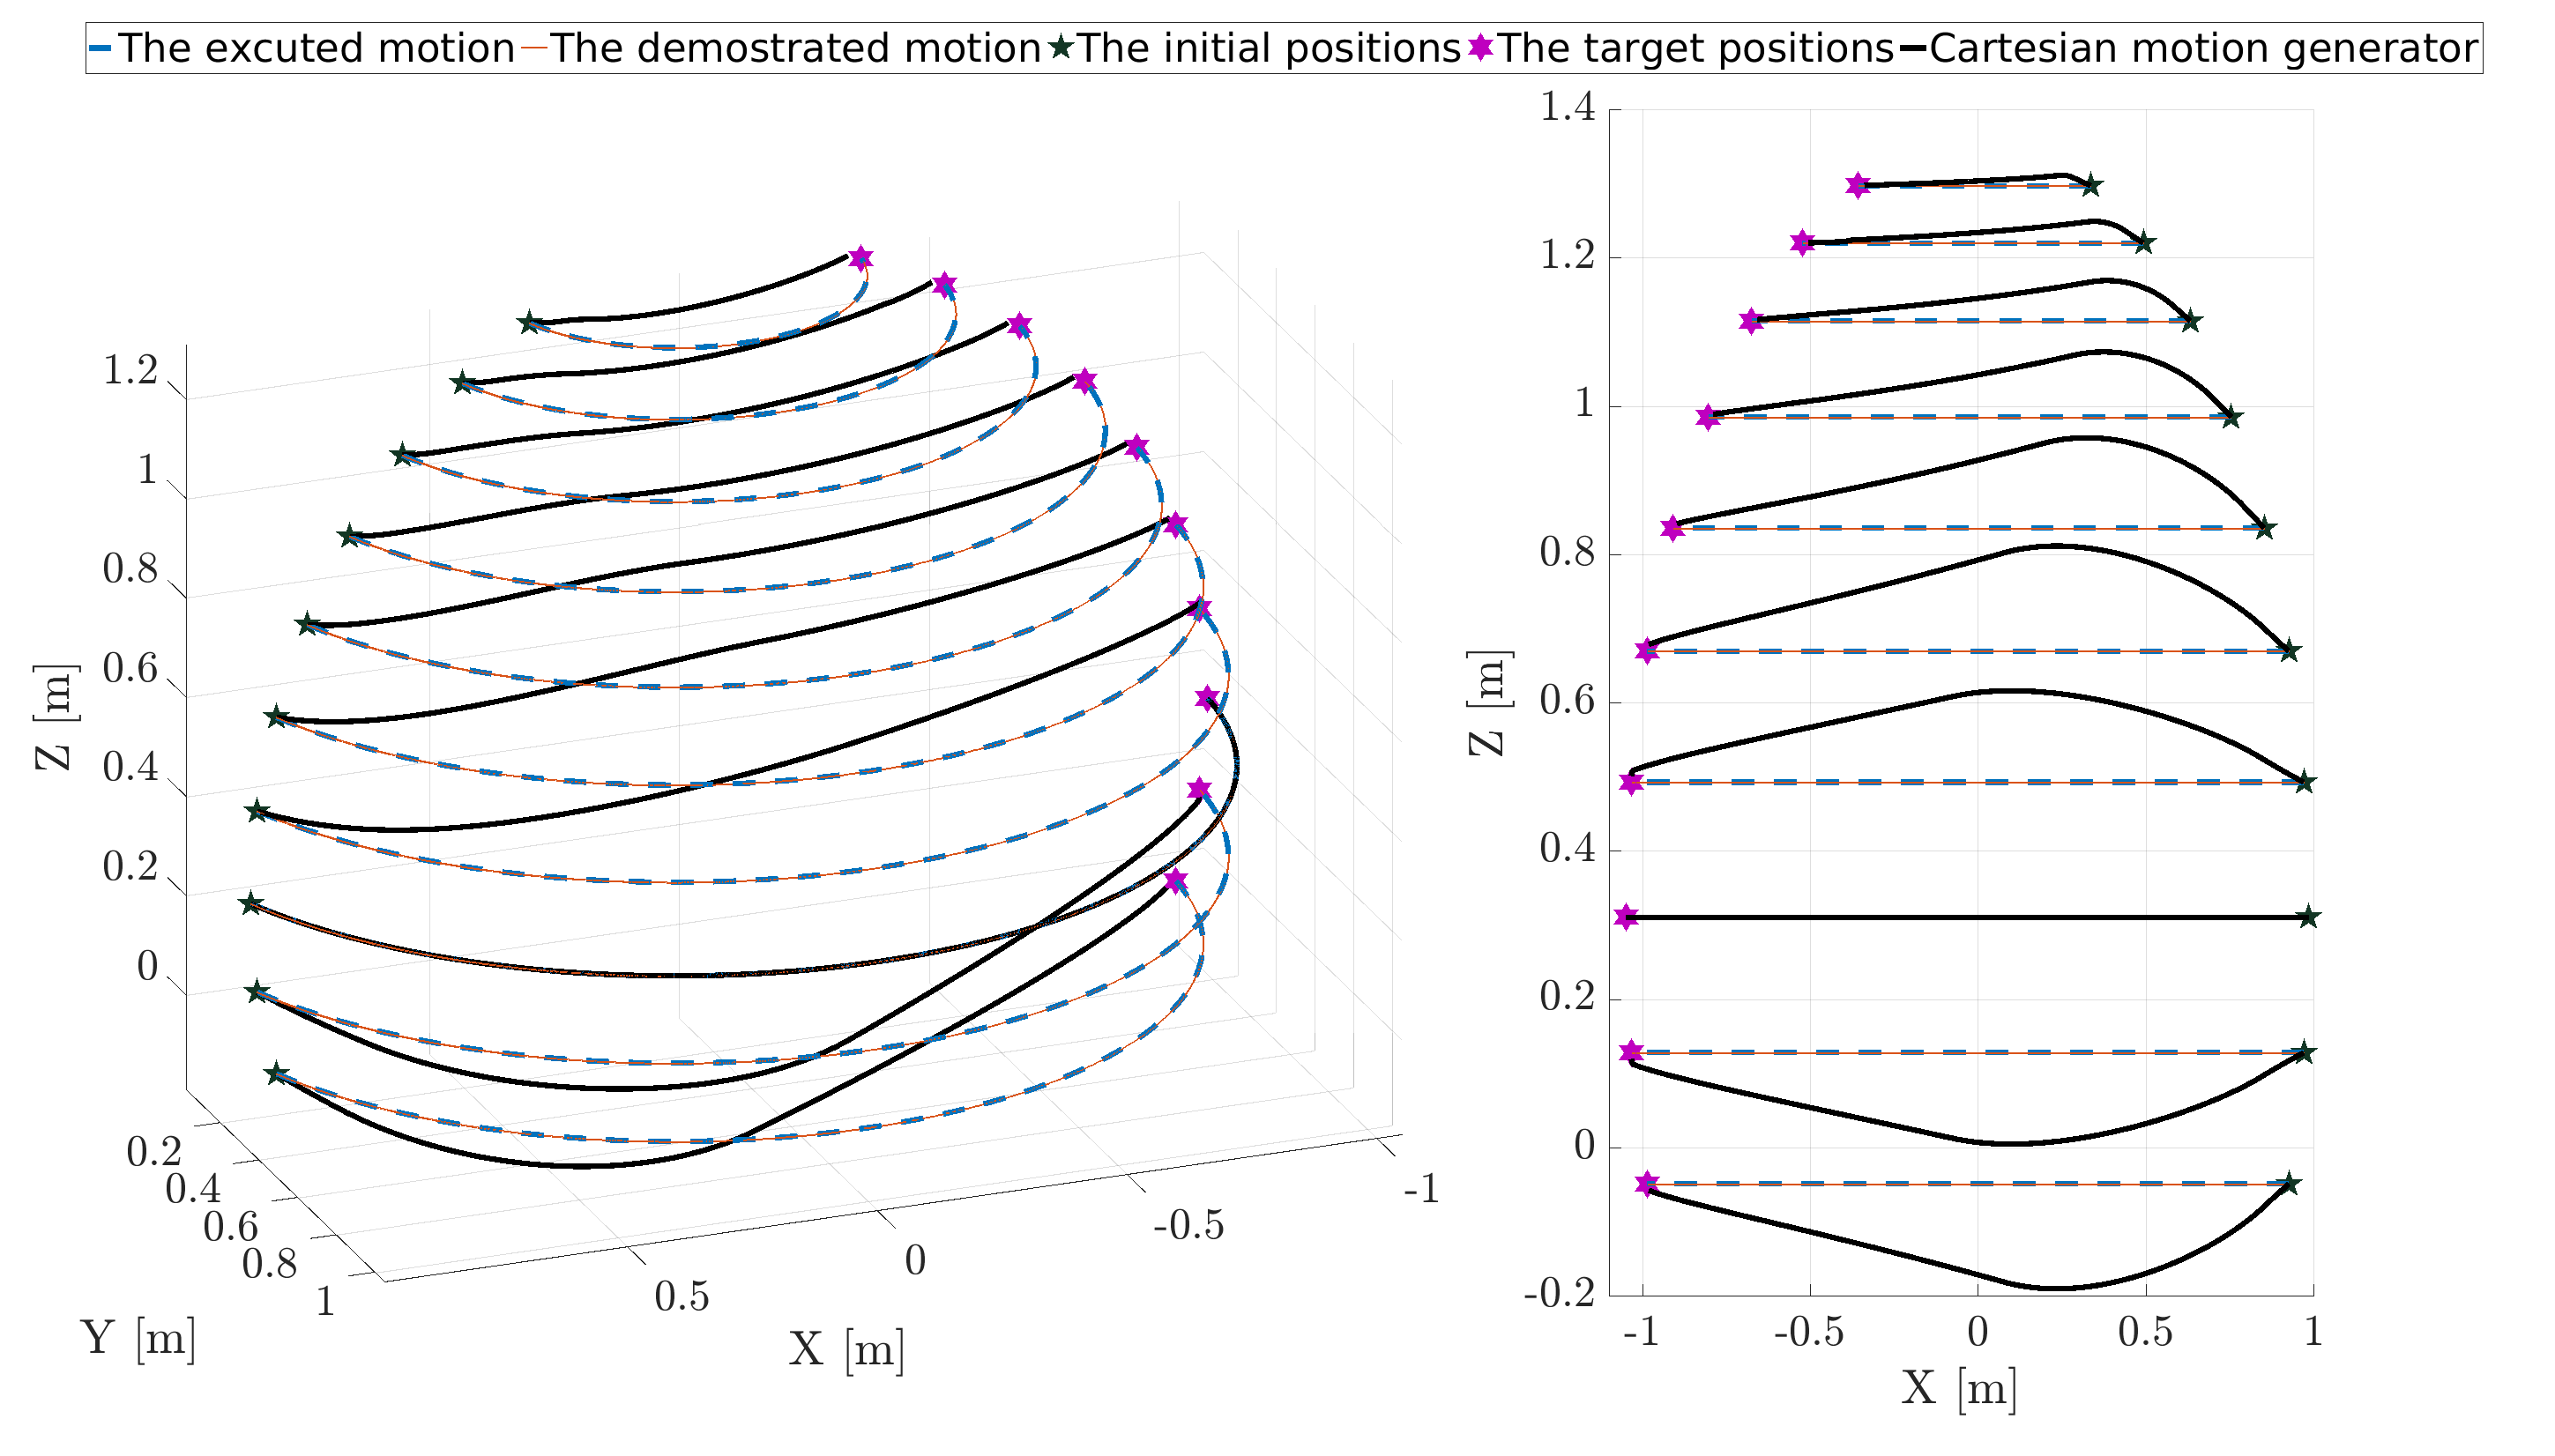
\includegraphics[width=\linewidth]{./figures/cropped_Sing_1.pdf}
	\caption{The experiment generated $K=3$ Gaussian components. As the first joint is the only joint which was not fixed during the demonstration, the learned augmentation matrices had only one nonzero entry $A_k(1,1)\neq0~\forall k\in \{1, 2, 3\} $.  In (a), the end-effector positions for the demonstrations and executed motions are plotted in Cartesian space. The JT-DS trajectory was generated closed-loop, while the SEDS trajectory was generated open-loop (otherwise it would be unstable).}
			\label{fig:Sin}
	\vspace{-20pt}
\end{figure}

Since we learn a lower-dimensional embedding space $Z := \{\phi(q) ~|~q \in Q\}$, which we suggest provides a better representation for the learned joint behaviors, a careful reader might wonder: why not define a motion policy $\pi_Z$ directly in $Z$-space and then map the learned policy back out into joint space using the inverse embedding $\phi^{-1}(z)$? The answer is that we would lose any guarantee of stability with respect to a target attractor $x_t^*$. By construction, $\phi$ maps from a joint-position vector of size $d$ to a low-dimensional vector of size $u<d$. Thus the inverse $\phi^{-1}$ must be of less than full rank, so the resulting $\mathcal{A}$ matrix (derived as in \eqref{eq:ds}) will also be of less than full rank, and thus no longer positive definite. This means that our controller no longer provably converges to the attractor (since our convergence proof no longer holds). Intuitively, this is because any policy defined in a lower-dimensional space than the actuation space will forfeit certain degrees of freedom, and thus may not be able to span the configuration space. Instead, we use the embedding space to modulate synergies defined in joint space, which we can guarantee will be positive definite and lead us to convergence to the target.

Finally,  we are currently working on improving the performance of the proposed DS, by learning its parameters wrt. the kinematic constraints. In this way, we can ensure that the performance of the DS is kinematically feasible for the robot to  follow.


{\footnotesize
\appendices
\section{Proving Stability of the Dynamical System}
\label{appendix:stability}
%We wish to prove Proposition \ref{prop:stability}, that is, that JT-DS \eqref{eq:ds} (reproduced below)
%\begin{equation*}
%\dot{q} = f(q) = -\mathcal{A}(q)J^T(q)P(H(q) - x^*)
%\end{equation*}
%accomplishes criterion (I), where $\mathcal{A}(q)$ is positive definite, and $P$ is positive definite.
%\newtheorem{theorem}{Theorem}[section]
%\begin{theorem}[Proof of Lyapunov Stability]
JT-DS \eqref{eq:ds} is asymptotically stable with respect to the Lyapunov candidate
\[ V(q) = \frac{1}{2}(H(q) - x^*)^T(H(q) - x^*) \]
That is, $ 0 \prec V(q),~ \forall q \neq q^*$ and $ V(q^*) = 0 $, where $q^*$ is any joint configuration such that $H(q^*) = x^*$.  The derivative of $ V $ wrt. time is:
\begin{equation}
\begin{aligned}
\frac{dV(q)}{dt} &= (H(q) - x^*)^TJ(q)\dot{q}\\
&= -(H(q) - x^*)^TJ(q)\mathcal{A}(q)J^T(q)(H(q) - x^*)\\
&= -(H(q) - x^*)^TJ(q)\sum_{k=1}^{K}\underbrace{\theta_k(\phi(q))}_{> 0}\underbrace{A_k}_{\succ 0}J^T(q)(H(q) - x^*)\leq 0
\end{aligned}
\end{equation}
When $J(q)$ is full-rank, the above inequality can be tightened to $\frac{dV(q)}{dt} < 0$. Therefore, as $ q=q^* $ is the largest invariance in $ \mathbb{R}^m $, JT-DS \eqref{eq:ds} is stable with respect to a task-space attractor; i.e. $\lim\limits_{t\rightarrow \infty} \| H(q)-x^*\|=0 $, and asymptotically stable for all regions in which the end-effector is fully manipulable ($J(q)$ is full rank).
}
\section*{Acknowledgment}
\footnotesize
The authors would like to thank A. Karimi for his insightful comments about formulating the convex optimization problem.

\bibliographystyle{IEEEtran}
% argument is your BibTeX string definitions and bibliography database(s)
\bibliography{IEEEabrv,references}
%



% that's all folks
\end{document}


